\documentclass[pdflatex,sn-mathphys,Numbered]{sn-jnl}

\usepackage{graphicx}
\usepackage{booktabs}
\usepackage{amsmath,amssymb,amsfonts}
\usepackage[title]{appendix}
\usepackage{longtable}
\hypersetup{colorlinks=true, linkcolor=blue, citecolor=blue, urlcolor=blue, pdftitle={Instruction-Fuel Drift, Boundary-Crossing Overhead, and Memory Safety in WebAssembly Sandboxes}, pdfauthor={Devarsh Patel}, pdfkeywords={WebAssembly, serverless computing, sandboxing, fuel metering, runtime benchmarking, WASI, measurement methodology}}
\usepackage{adjustbox}
\usepackage{array}
\renewcommand{\topfraction}{0.92}
\renewcommand{\bottomfraction}{0.85}
\renewcommand{\textfraction}{0.07}
\renewcommand{\floatpagefraction}{0.80}
\setcounter{topnumber}{3}
\setcounter{bottomnumber}{2}
\setcounter{totalnumber}{4}
\newtheorem{proposition}{Proposition}

\begin{document}

\title[Instruction-Fuel Drift in WebAssembly Sandboxes]{Instruction-Fuel Drift, Boundary-Crossing Overhead, and Memory Safety in WebAssembly Sandboxes: A Multi-Runtime Measurement Study}

\author[1]{\fnm{Devarsh} \sur{Patel}}\email{devarsh.patel2024@vitstudent.ac.in}
\author*[1]{\fnm{Ranjithkumar} \sur{S}}\email{ranjithkumar.s@vit.ac.in}

\affil*[1]{\orgdiv{School of Computer Science and Engineering (SCOPE)}, \orgname{Vellore Institute of Technology (VIT)}, \orgaddress{\city{Vellore}, \state{Tamil Nadu}, \country{India}}}

\abstract{
Multi-tenant WebAssembly platforms bound tenant CPU with instruction fuel. We measure how closely fuel tracks the CPU time a tenant consumes, how that relation depends on the runtime and the build, and what the sandbox boundary costs. The corpus has 50 kernels (30 PolyBench/C, 10 integer and cryptographic, and 10 linear-memory kernels) at four frontend optimization levels, giving 200 cells. We time each cell under twelve runtime configurations on an 8-core Apple M3 system-on-chip and obtain 166{,}600 timed replicates. All configurations return identical checksums in every cell. Under Wasmtime's Cranelift backend the cost of one fuel unit varies by a factor of $40.8$ across cells, while a robust 95th-to-5th percentile ratio of $8.9$ shows that most cells are closer together than the extremes suggest. The same kernel's fuel differs by factors from $0.36$ to $6.5$ between $-$O0 and $-$O2 builds, and Winch and Cranelift disagree on fuel in 20 cells above numerical noise. Across 4{,}800 single-operation linear-memory probes every outcome conformed, with an exact 95\% lower bound of $0.995$ on conformance for each configuration. Sandbox recycling adds about 9 bytes of private anonymous memory per lifecycle, independently of the sandbox's dirty pages and of the allocation strategy. A host call costs about 61 times a native copy-and-validate at 64-byte payloads and reaches parity at 4\,MiB, and WASI Preview 2 writes cost less per byte than Preview 1 writes. Calibrating cost per fuel unit with opcode-class counts, whether static or dynamically executed, does not reduce dispersion below the uncalibrated fuel baseline.
}

\keywords{WebAssembly, serverless computing, sandboxing, fuel metering, runtime benchmarking, WASI, measurement methodology}

\maketitle

\section{Introduction}
\label{sec:intro}
Multi-tenant platforms run untrusted code in WebAssembly sandboxes because the sandbox starts quickly and isolates memory \cite{haas2017bringing, shillaker2020faasm}. Memory isolation is only part of the contract. A host also needs a bound on the CPU a tenant can consume, and most WebAssembly runtimes supply one by metering instructions. The meter is called fuel. The runtime decrements fuel as the guest executes and traps when the budget runs out.

Fuel counts guest operations, while CPU time depends on the machine code the runtime emits for them. Two compilers sit between the two: the frontend that produces the module, and the backend that lowers it to native code. Both change the work a fixed source computation performs, and the backend changes what each operation costs. A fixed fuel budget therefore buys different CPU time on different modules, optimization levels, and runtimes. Jangda et al.\ measured WebAssembly against native code across a benchmark suite \cite{jangda2019not}. The question here is narrower: how closely does metered fuel approximate the time a tenant consumes, and how much does that approximation depend on the runtime and the build?

We make five key contributions:
\begin{itemize}
\item \textbf{Fuel-to-time drift and backend dependence.} For 50 kernels at four optimization levels we quantify the cost of one fuel unit across cells, and we show that the Winch and Cranelift backends report different fuel for the same module (Section~\ref{sec:rq1}).
\item \textbf{Cross-runtime cost with metering overhead.} We time all 200 cells under twelve configurations, including metered and unmetered builds of three Wasmer backends and both the interpreter and ahead-of-time modes of WasmEdge. All configurations return identical checksums (Section~\ref{sec:rq1}).
\item \textbf{Trap conformance.} We run 4{,}800 single-operation linear-memory probes under six memory configurations, and all of them conform (Section~\ref{sec:rq2}).
\item \textbf{Host-boundary and WASI cost.} We fit cost models to a custom host-call boundary and to WASI Preview 1 and Preview 2 writes, from 12{,}964 host samples and 12{,}964 WASI invocations (Section~\ref{sec:rq3}).
\item \textbf{Recycling and a negative calibration result.} Sandbox recycling produces a stable growth term that is independent of sandbox dirty pages. Calibration with static and with dynamically executed opcode-class counts does not reduce dispersion, and we report the failure with its evidence (Section~\ref{sec:rq4}, Section~\ref{sec:rq5}).
\end{itemize}
Section~\ref{sec:discussion} turns these results into guidance for operators who set tenant budgets in fuel.

Section~\ref{sec:related} reviews prior work, and Section~\ref{sec:metrics} defines the metrics and the decomposition used in the analysis. Section~\ref{sec:methods} describes the testbed and telemetry, Section~\ref{sec:results} reports the five research questions, and Section~\ref{sec:discussion} turns them into guidance for operators. Section~\ref{sec:conclusion} concludes.

\section{Related Work}
\label{sec:related}
The 44 bibliography entries comprise WebAssembly foundations and runtime studies from 2017 to 2020, recent runtime, security, and WASI work from 2024 to 2026, and the statistical and methodology references from 1934 to 2009 that Section~\ref{sec:metrics} uses. Table~\ref{tab:lit_taxonomy} places the closest empirical studies side by side, and the five clusters below group the rest.
The search protocol ran ten keyword searches restricted to 2024 onward and six saturation checks that count recent papers on a candidate gap. Together they returned 124 records. Thirty-two were repeats of a record already seen, which left 92 unique records. A record was kept only if it was a peer-reviewed article or conference paper from an established publisher or indexed proceedings, and only if its topic was runtime performance, sandbox isolation, host interfaces, or measurement methodology. Theses, preprints, repository copies, and papers from venues outside the indexed databases were excluded. That left 28 records, 19 of which were already in the verified reference list from an earlier pass. The other nine were added after their Crossref metadata matched their titles. The decision for every record is logged in the repository. The search index covers paywalled and open-access work alike, but its ranking favours recent and highly cited papers, so the search can miss a relevant paper that is neither.

Each bibliography entry was checked against its Crossref or USENIX record for title, year, venue, and pages. The cluster descriptions state each work's scope and reported results.

We group the works into five clusters. The grouping is ours.

\textbf{Cluster A: runtimes and cross-platform evaluation.} Zhang et al.\ survey 103 research papers on WebAssembly runtimes, covering runtime design, testing, and application domains \cite{zhang2025survey}. Khan et al.\ evaluate 13 WASI-compatible runtimes on eight machine-learning and arithmetic benchmarks, with an external power meter, and report that interpreter-oriented runtimes exceed $10\times$ overhead in time and energy while optimized AOT engines approach a native reference \cite{khan2026taxonomy}. Moron and Wallentowitz benchmark WebAssembly on microcontrollers against native code, MicroPython, and Lua \cite{moron2025embedded}. Kakati and Brorsson evaluate two runtimes across four architectures, including RISC-V and embedded boards, for speed and startup time \cite{kakati2024cross}, and a later conference paper addresses the performance and usability of multiplatform WebAssembly containers \cite{kakati2025multiplatform}. Khelifa et al.\ find roughly $1.1\times$ overhead for small deep-learning networks on standalone runtimes, with larger networks showing greater overhead \cite{khelifa2024case}. De Palma et al.\ benchmark a WebAssembly function-as-a-service platform against three container-based platforms on constrained edge hardware \cite{depalma2024webassembly}. Khan et al.\ compare machine-learning programs written in Python, Rust, and C++ and compiled to WebAssembly, in a browser and under WASI \cite{khan2025ml}. Golec et al.\ survey cold-start latency in serverless computing and propose a taxonomy of mitigations \cite{golec2025cold}. Moebius et al.\ compare unikernels with Firecracker microVMs, Docker, and gVisor for cold start and idle footprint at the edge \cite{moebius2024unikernels}. Chennubhotla et al.\ report that WebAssembly configurations run 31.4\% faster, use 59.5\% less memory, and produce images 86.5\% smaller than Docker \cite{chennubhotla2025docker}.

\textbf{Cluster B: security, isolation, and resource control.} Perrone and Romano review 121 papers on WebAssembly security, organized into seven categories \cite{perrone2025security}. Draissi et al.\ analyze memory corruption in WebAssembly across 37{,}797 web domains and find that 77.81\% of them fully trust data that attacker-controlled sources can influence \cite{draissi2025wemby}. Wang et al.\ virtualize WebAssembly linear memory for enclaves to allow page-level sharing and access control \cite{wang2025waven}. Rostamipoor et al.\ protect serverless functions against memory-leakage attacks with selective encryption and report overheads of 2.8\% to 8.5\% \cite{rostamipoor2025leakless}. Yu et al.\ decouple the WASI system interface into a virtualized daemon, which costs a $3.2\times$ slowdown on the WASI call path but gives three times the memory density of Firecracker \cite{yu2026wasc}. Coppolino et al.\ build a multi-tenant embedded runtime with a patched system interface and a trusted execution environment \cite{coppolino2025wasmbox}. Fink et al.\ use Arm memory tagging and pointer authentication for WebAssembly memory safety, with runtime overheads below 5.8\% \cite{fink2025cage}. Yu et al.\ report that current runtimes do not protect resource isolation well: a malicious instance can exhaust host resources through the WASI and WASIX interfaces, and they derive exploitation strategies from static analysis of the runtimes \cite{yu2025resource}. Fuel meters guest operations, so host-side work that a guest reaches through WASI calls is outside the budget this paper measures. The foundations are Narayan et al.\ on fine-grained isolation in a production browser \cite{narayan2020firefox}, Lehmann et al.\ on the binary security of WebAssembly \cite{lehmann2020binary}, Shillaker and Pietzuch on stateful serverless isolation \cite{shillaker2020faasm}, and Agache et al.\ on lightweight virtualization for serverless \cite{agache2020firecracker}.

\textbf{Cluster C: instrumentation, compilers, and testing.} Titzer et al.\ present non-intrusive dynamic instrumentation for WebAssembly, with probes that can be inserted and removed and that cost nothing when disabled \cite{titzer2024flexible}. That is the mechanism a dynamic calibration would need, and Section~\ref{sec:rq5} uses the same counting idea. Schwarz et al.\ present TPDE, a single-pass back-end framework that compiles LLVM IR 8 to 26 times faster than LLVM at $-$O0 with run-time performance on par with it \cite{schwarz2026tpde}. Tamura et al.\ add ahead-of-time instrumentation to WebAssembly for cross-ISA checkpoint and restore, with an average execution overhead of 36\% \cite{tamura2025bringing}. Jiang et al.\ generate runtime performance test programs with a distinguishability measure \cite{jiang2025warpgen}, and Zeng et al.\ locate the instructions behind runtime performance issues by mutation-based inference \cite{zeng2026warpl}.

\textbf{Cluster D: host interfaces and WASI.} Mao et al.\ instrument WASI calls with eBPF and measure total time, startup, WASI time, and syscall time under I/O load \cite{mao2024ewapa}. Van Kenhove et al.\ add I2C and USB interfaces to WebAssembly, with at most 8\% overhead against native USB APIs and a runtime-initialization cost that matters at low latency \cite{vankenhove2025cyberphysical}. Seidler et al.\ run device drivers inside WebAssembly containers and report lower latency and overhead than user-level drivers \cite{seidler2025wasmio}. Ramesh et al.\ propose thin kernel interfaces for WebAssembly, arguing that the missing standard system interfaces slow adoption \cite{ramesh2025thin}. Jansen et al.\ integrate the WebAssembly Micro Runtime into a container runtime, reducing memory per container by 11\% to 78\% against existing WebAssembly runtimes \cite{jansen2025memory}.

\textbf{Cluster E: methodology and statistics.} Antunes and Hill survey reproducibility in high-performance computing \cite{antunes2024reproducibility}, and Pearce et al.\ define repeat, replicate, and reproduce for benchmarking runs \cite{pearce2025hpc}. Lema et al.\ compare deep-learning detectors with analysis of variance and Tukey tests on a small dataset, and they show that reported gains are often not significant \cite{lema2026benchmarking}. Mytkowicz et al.\ show that measurement setup can change conclusions \cite{mytkowicz2009wrong}, and Georges et al.\ set out statistically rigorous performance evaluation \cite{georges2007java}. The statistical methods are the Clopper--Pearson interval \cite{clopper1934use}, Welch's ANOVA \cite{welch1951comparison}, ridge regression \cite{hoerl1970ridge}, and the peaks-over-threshold generalized Pareto model \cite{davison1990exceedances}.

Across the five clusters, three structural gaps motivate the experimental design. In the screened set, they are as follows.
\begin{enumerate}
\item \textbf{Absence of cross-backend fuel-to-time auditing.} Prior studies compare wall-clock speed, energy, and startup across runtimes \cite{jangda2019not, khan2026taxonomy, kakati2024cross}, or measure host resource exhaustion through WASI and WASIX \cite{yu2025resource}. None quantifies how closely a runtime's internal instruction-fuel meter tracks on-CPU time across frontend optimization levels (\texttt{-O0} through \texttt{-Oz}) and backend code generators (Cranelift, Winch, Singlepass, LLVM, and AOT). The search for the fuel meter returned almost nothing recent, although a narrow query can miss vocabulary.
\item \textbf{Unquantified WASI Preview 1 versus Preview 2 per-byte scaling.} WASI evaluations report aggregate application or eBPF syscall shares \cite{mao2024ewapa, yu2026wasc}. None decomposes host-function and WASI Preview 1 (\texttt{wasm32-wasip1}) and Component Model Preview 2 (\texttt{wasm32-wasip2}) writes into a fixed boundary cost and a marginal per-byte slope inside one engine. Host-call costs are reported as percentages rather than as fixed and marginal costs.
\item \textbf{No load-gated multi-allocator recycling study and no tested dynamic calibration.} Container and sandbox density studies \cite{jansen2025memory, shillaker2020faasm} do not isolate per-lifecycle private memory growth across on-demand and pooling allocators under a verified wall-to-CPU contention gate. Dynamic instrumentation \cite{titzer2024flexible} makes opcode counting possible, but no screened study tests whether such counts calibrate away fuel-to-time dispersion. Load control and a wall-versus-CPU check are not reported for WebAssembly benchmarks in the screened set.
\end{enumerate}
\begin{table}[t]
\caption{Taxonomic comparison of this study against representative empirical WebAssembly runtime, security, and WASI studies. Entries summarize the scope described for each work in Section~\ref{sec:related}. A dash means that the work does not report that measurement.}\label{tab:lit_taxonomy}
\footnotesize
\setlength{\tabcolsep}{3pt}%
\begin{adjustbox}{max width=\textwidth}%
\begin{tabular}{lllllllll}
\toprule
Study & Venue (year) & Runtimes & Opt.\ levels & Fuel drift & Backend fuel & Guard probes & WASI P1 vs.\ P2 & Recycling \\
\midrule
Haas et al.~\cite{haas2017bringing} & PLDI 2017 & Browsers & --- & --- & --- & --- & --- & --- \\
Jangda et al.~\cite{jangda2019not} & USENIX ATC 2019 & Browsers (2) & --- & --- & --- & --- & --- & --- \\
Shillaker \& Pietzuch~\cite{shillaker2020faasm} & USENIX ATC 2020 & Faasm (Wasm SFI) & --- & --- & --- & --- & Faaslet host interface & Snapshot restore \\
Lehmann et al.~\cite{lehmann2020binary} & USENIX Security 2020 & --- & --- & --- & --- & --- & --- & --- \\
Titzer et al.~\cite{titzer2024flexible} & ASPLOS 2024 & Wizard engine & --- & Dynamic probes & --- & --- & --- & --- \\
Kakati \& Brorsson~\cite{kakati2024cross} & CCGrid 2024 & 2 runtimes, 4 ISAs & --- & --- & --- & --- & --- & Startup time \\
Mao et al.~\cite{mao2024ewapa} & SSE 2024 & --- & --- & --- & --- & --- & eBPF WASI trace & --- \\
Khan et al.~\cite{khan2026taxonomy} & IEEE Access 2026 & 13 WASI runtimes & --- & --- & --- & --- & --- & --- \\
Yu et al.~\cite{yu2025resource} & USENIX Security 2025 & --- & --- & --- & --- & --- & Host exhaustion via WASI/WASIX & --- \\
Jansen et al.~\cite{jansen2025memory} & IPDPSW 2025 & WAMR in containers & --- & --- & --- & --- & --- & Memory footprint \\
Yu et al.~\cite{yu2026wasc} & ACM TACO 2026 & WaSC daemon & --- & --- & --- & --- & Decoupled WASI daemon & Multi-tenant density \\
\midrule
\textbf{This study} & \textbf{2026} & \textbf{12 configurations} & \textbf{4 (\texttt{-O0}--\texttt{-Oz})} & \textbf{Yes ($40.8\times$)} & \textbf{Yes (20 cells)} & \textbf{Yes (4,800 probes)} & \textbf{Yes (64\,B--16\,MiB)} & \textbf{Yes (1.68M lifecycles)} \\
\bottomrule
\end{tabular}%
\end{adjustbox}
\end{table}


\section{Metrics and Models}
\label{sec:metrics}
\label{sec:models}
Let a cell $c=(k,o)$ be kernel $k$ built at optimization level $o$. For one timed \texttt{run(reps)} call $r$ in cell $c$, let $F(r)$ be the fuel the runtime reports for that call and $C(r)$ the thread CPU time in nanoseconds. The cost of one fuel unit is
\begin{equation}
\psi(r) = \frac{C(r)}{F(r)} \quad [\mathrm{ns\,per\,fuel\,unit}],
\end{equation}
and $\mu_\psi(c)$ is its mean over the replicates of $c$. The adversarial amplification factor of a metered runtime $b$ is
\begin{equation}
\mathcal{A}_{\mathrm{adv}}(b) = \frac{\max_{c}\,\mu_{\psi}(b,c)}{\min_{c}\,\mu_{\psi}(b,c)}.
\end{equation}
A tenant that chooses its kernel and build can convert a fixed fuel budget into CPU time at a rate that varies by this factor. The factor is set by two extreme cells, so we also report the ratio of the 95th to the 5th percentile of $\mu_\psi$, and the interquartile ratio, as robust spreads.

Fuel is a runtime-specific counter. Wasmer's metering middleware charges one unit per operator in our configuration. WasmEdge's instruction counter counts executed instructions. Wasmtime reports its own consumed-fuel count, which we use as given. We treat each meter as the fuel of its runtime and do not assume that two of them measure the same thing.

Trap conformance is the fraction of probes whose outcome matches the specification, where a graceful trap and a specified return both count as conforming. The interval is the exact Clopper--Pearson binomial interval \cite{clopper1934use}. Cross-level differences in time are tested with Welch's heteroscedastic ANOVA on log-transformed times \cite{welch1951comparison}, and we report partial $\eta^2$ computed from the Welch $F$ statistic. Recycling growth is the OLS slope of memory against lifecycle count, and the lifecycle latency tail is summarized by a generalized Pareto fit to exceedances over the 95th percentile \cite{davison1990exceedances}. Host-call cost is modeled as
\begin{equation}
T(s) = \alpha + \beta s,
\end{equation}
where $s$ is payload size in bytes, fitted by ordinary least squares with $t$-based intervals.

The calibration model predicts a cell's mean time from opcode-class counts. Row $i$ of $X$ holds the counts for cell $i$, and $t_i$ is its measured mean time. The ridge estimate is
\begin{equation}
\hat{u} = \arg\min_{u \ge 0}\; \lVert X u - t \rVert_2^2 + \lambda \lVert u - \mathbf{1} \rVert_2^2 ,
\end{equation}
with the prior $u=\mathbf{1}$ meaning a uniform cost per opcode class \cite{hoerl1970ridge}. The model is scored by leave-one-cell-out prediction: each cell's prediction uses weights fitted without that cell, and dispersion is the coefficient of variation of time divided by that prediction. Two designs are compared. The static design counts instruction lines in the disassembled function bodies. The dynamic design counts the instructions that actually execute, which we measured by instrumentation (Section~\ref{sec:methods}).

\subsection{Microarchitectural decomposition and a linear recalibration bound}
\label{subsec:decomposition}
Fuel counts executed operations, while CPU time depends on the cycles those operations take. This subsection writes the relation explicitly, so that the limits of any calibration based on operator classes can be stated and checked against the data. Let $\mathcal{D}$ index the $D$ operator classes, let $N_{c,d}$ be the executed count of class $d$ in cell $c$, and let $N_c=\sum_{d}N_{c,d}$. Let $N_{c,\mathrm{mem}}$ and $N_{c,\mathrm{br}}$ count memory and branch operations. On an out-of-order core at effective clock $f_{\mathrm{eff}}$, the on-CPU time of a cell, Eq.~\eqref{eq:cpi_decomp}, is the sum of base execution cycles and stall cycles from the memory hierarchy and from branch recovery:
\begin{equation}\label{eq:cpi_decomp}
C(c)=\frac{1}{f_{\mathrm{eff}}}\Bigl(\sum_{d=1}^{D}N_{c,d}\,\gamma_{0,d}+N_{c,\mathrm{mem}}\sum_{\ell\in\{\mathrm{L1D},\mathrm{L2},\mathrm{SLC}\}}m_{c,\ell}\,\tau_{\ell}+N_{c,\mathrm{br}}\,b_{c,\mathrm{miss}}\,\tau_{\mathrm{br}}\Bigr).
\end{equation}
Here $\gamma_{0,d}$ is the base cycle cost of class $d$ when every access hits in L1, $m_{c,\ell}\in[0,1]$ is the miss rate of cell $c$ at level $\ell$ with penalty $\tau_{\ell}$, and $b_{c,\mathrm{miss}}$ is the branch misprediction rate with flush penalty $\tau_{\mathrm{br}}$. Dividing by $N_c$ and writing $p_{c,d}=N_{c,d}/N_c$, $p_{c,\mathrm{mem}}=N_{c,\mathrm{mem}}/N_c$, and $p_{c,\mathrm{br}}=N_{c,\mathrm{br}}/N_c$ for the dynamic shares gives the cost per fuel unit $\mu_\psi(c)=C(c)/N_c$ as
\begin{equation}\label{eq:psi_decomp}
\mu_\psi(c)=\underbrace{\frac{1}{f_{\mathrm{eff}}}\sum_{d=1}^{D}p_{c,d}\,\gamma_{0,d}}_{\text{class-mix term}}+\underbrace{\frac{1}{f_{\mathrm{eff}}}\Bigl(p_{c,\mathrm{mem}}\sum_{\ell}m_{c,\ell}\,\tau_{\ell}+p_{c,\mathrm{br}}\,b_{c,\mathrm{miss}}\,\tau_{\mathrm{br}}\Bigr)}_{\text{state-dependent stall residual }\Delta(c)}.
\end{equation}
The class-mix term is linear in the shares. The stall residual depends on miss and misprediction rates, which describe the memory and branch state a cell produces and not the operators it executes.

Stack the costs of the $n$ cells in a vector $\boldsymbol{\mu}$, and let $\mathbf{P}\in\mathbb{R}^{n\times(D+1)}$ be the design matrix whose first column is a vector of ones and whose remaining columns are the class shares. Let $\mathbf{P}_{\mathrm{mix}}$ hold the share columns alone, let $\boldsymbol{\Delta}$ stack the stall residuals, and let $\mathbf{H}$ be the orthogonal projector onto the column space of $\mathbf{P}$. The effective clock is treated as common to all cells, which the reported range of $3.65$ to $3.73$\,GHz permits. If it varied by cell, that variation would enter $\boldsymbol{\Delta}$.

\begin{proposition}[Linear recalibration bound]\label{prop:linear_bound}
(i) For every $\mathbf{u}\in\mathbb{R}^{D+1}$,
\begin{equation*}
\|\boldsymbol{\mu}-\mathbf{P}\mathbf{u}\|_2^2\ \ge\ \|(\mathbf{I}-\mathbf{H})\boldsymbol{\mu}\|_2^2=(1-R^2)\,\|\boldsymbol{\mu}-\bar{\mu}\mathbf{1}\|_2^2,
\end{equation*}
with equality when $\mathbf{P}\mathbf{u}=\mathbf{H}\boldsymbol{\mu}$, where $R^2$ is the in-sample coefficient of determination of the least-squares fit of $\boldsymbol{\mu}$ on $\mathbf{P}$ and $\bar{\mu}$ is the mean of $\boldsymbol{\mu}$. Consequently the residual $\boldsymbol{\mu}-\mathbf{P}\mathbf{u}$ has a sample coefficient of variation, relative to $\bar{\mu}$, of at least $\mathrm{CV}(\mu_\psi)\sqrt{1-R^2}$ for every linear recalibration by class counts.
(ii) Under Eq.~\eqref{eq:psi_decomp}, $\boldsymbol{\mu}=\mathbf{P}_{\mathrm{mix}}\mathbf{w}+\boldsymbol{\Delta}$ for a fixed weight vector $\mathbf{w}$, and $(\mathbf{I}-\mathbf{H})\boldsymbol{\mu}=(\mathbf{I}-\mathbf{H})\boldsymbol{\Delta}$. The part of the cost per fuel unit that no class-count recalibration can remove is therefore the part of the stall residual that lies outside the span of the class shares.
\end{proposition}

\begin{proof}
For (i), $\mathbf{H}\boldsymbol{\mu}-\mathbf{P}\mathbf{u}$ lies in the column space of $\mathbf{P}$, and $(\mathbf{I}-\mathbf{H})\boldsymbol{\mu}$ is orthogonal to that space. The Pythagorean identity gives $\|\boldsymbol{\mu}-\mathbf{P}\mathbf{u}\|^2=\|(\mathbf{I}-\mathbf{H})\boldsymbol{\mu}\|^2+\|\mathbf{H}\boldsymbol{\mu}-\mathbf{P}\mathbf{u}\|^2$, and the second term vanishes at $\mathbf{P}\mathbf{u}=\mathbf{H}\boldsymbol{\mu}$. Because the first column of $\mathbf{P}$ is $\mathbf{1}$, $(\mathbf{I}-\mathbf{H})\mathbf{1}=\mathbf{0}$, so $\|(\mathbf{I}-\mathbf{H})\boldsymbol{\mu}\|^2=\|\boldsymbol{\mu}-\bar{\mu}\mathbf{1}\|^2-\|\mathbf{H}(\boldsymbol{\mu}-\bar{\mu}\mathbf{1})\|^2$, and the last term equals $R^2\|\boldsymbol{\mu}-\bar{\mu}\mathbf{1}\|^2$. The residual sum of squares is therefore at least $(1-R^2)$ times the total sum of squares. Dividing both by $n-1$ and taking square roots gives a residual standard deviation of at least $\sqrt{1-R^2}\,\mathrm{sd}(\boldsymbol{\mu})$, and dividing by $\bar{\mu}$ gives the coefficient-of-variation bound. For (ii), $\mathbf{P}_{\mathrm{mix}}\mathbf{w}$ lies in the column space of $\mathbf{P}$, so $\mathbf{I}-\mathbf{H}$ annihilates it.
\end{proof}

Proposition~\ref{prop:linear_bound} is a statement about in-sample fits, and it holds whatever the quality of the class counts as predictors. Its use here is to measure how much of the dispersion the class counts can account for at all. Table~\ref{tab:rq5_bound} reports the measured $R^2$ on the 200 Cranelift cells. The class shares explain $18.2\%$ of the variance of $\mu_\psi$ in the dynamic case and $24.4\%$ in the static case, so no linear recalibration in sample can bring the residual coefficient of variation below $0.889$ and $0.854$. The leave-one-cell-out results in Section~\ref{sec:rq5} are worse than these bounds, as expected for out-of-sample predictions. The bound applies to the additive residual. The score in Section~\ref{sec:rq5} is the coefficient of variation of time divided by prediction, which is multiplicative, so the bound is a benchmark and not a bound on the reported score.

\section{Testbed and Telemetry Architecture}
\label{sec:methods}
\subsection{Hardware, toolchain, and corpus}
All experiments ran on a Mac with an 8-core Apple M3 system-on-chip (ARMv8.6-A), four performance cores and four efficiency cores, under macOS 26.6.2 (build 25G83). The performance cluster has a 128\,KiB L1 data cache and a 16\,MiB shared L2 cache, and the efficiency cluster has a 64\,KiB L1 data cache and a 4\,MiB shared L2 cache. We state these capacities because the cache-capacity steps in the host-call sweep (Section~\ref{sec:rq3}) depend on them, and the counters described below are macOS interfaces. Kernels were compiled with LLVM 23.1.3 to the \texttt{wasm32-wasip1} target against wasi-libc and linked with lld. The WASI comparison (Section~\ref{sec:rq3}) also uses a \texttt{wasm32-wasip2} build of the same source. Every module exports \texttt{run(reps)}, which executes the workload, and \texttt{check()}, which returns an output checksum.

The 30 PolyBench/C 4.2.1 kernels are used unmodified at the MEDIUM dataset. A generated wrapper routes PolyBench's checksum dump into a hash so that output equality can be checked across runtimes. The ten integer and cryptographic kernels are CRC-32, Collatz, division and remainder, cache thrashing, FNV-1a, branch misprediction, quicksort, substring search, SHA-256, and ChaCha20. SHA-256 agrees with \texttt{hashlib} on the generated message, and the ChaCha20 block agrees with the RFC~7539 test vector. The ten linear-memory kernels cover streaming copy, pointer chasing, strided access at 64\,B and 4\,KiB, reduction, binary search, transposition, hash-table probing, growth to a fixed working set, and address wrap-around. These are memory-behavior kernels. They do not sweep WASI system calls. Every kernel is built at $-$O0, $-$O2, $-$O3, and $-$Oz, giving 200 cells. Appendix~\ref{app:corpus} gives the module sizes. A validation pass confirms that \texttt{check()} is deterministic and agrees across the four levels for every kernel, and that the SHA-256 and ChaCha20 kernels match their reference values.

\subsection{Runtimes}
Table~\ref{tab:campaign} lists the twelve timed configurations. Wasmtime 50.0.0 runs Cranelift and Winch through a Rust harness with fuel consumption enabled. Wasmer 7.5.0 runs Singlepass, Cranelift, and LLVM 22.1, each unmetered and metered with the operator-counting middleware. WasmEdge 0.18.0 runs in interpreter mode and in ahead-of-time mode, compiled with \texttt{wasmedgec} at optimization level 3 with the instruction counter enabled. WAMR (iwasm 2.4.5) runs its interpreter. Node.js 26.11.1 (V8 14.6) is a timing-and-counter engine without a fuel meter. Every runtime executes the same plan of cells and reps, calibrated once with Cranelift so that one call takes about 20\,ms.

\subsection{Telemetry}
Each timed replicate records thread CPU time (\texttt{CLOCK\_THREAD\_CPUTIME\_ID}), wall time, the runtime's fuel count where one exists, a checksum, and two hardware counters. The counters are the retired-instruction and core-cycle totals that \texttt{proc\_pid\_rusage} with \texttt{RUSAGE\_INFO\_V4} reports for the process. This interface does not require root privileges. The V8 harness reads the same counters through a small N-API addon. The counters are taken as reported. We did not validate them against a microbenchmark with a known instruction count, so we use them for comparisons between runtimes and as a consistency check on the effective clock.

Dynamic opcode counts come from a separate, untimed pass. Each module is disassembled, and a stack-neutral increment of a per-class global is placed before every instruction in the function bodies. The instrumented text is reassembled and run once with the cell's timing reps. The run returns the same value as the uninstrumented module in every cell, which was checked before the counts were used. The dynamic total agrees with Wasmtime's fuel to within $0.03\%$ in median.

\subsection{Protocol and load control}
Each cell receives two warm-up calls. The timed replicates run in a seeded random order over cells. The fast runtimes have 100 replicates per cell, Singlepass and WAMR have 10, and the WasmEdge interpreter has 3, because it runs about $90\times$ slower than Cranelift. The reduced counts widen those intervals.

Load control and telemetry gating protocols enforce strict execution isolation. The benchmarking harness gates each runtime sweep on load-average thresholds before every replicate to guarantee clean, idle execution windows. Telemetry tracks the wall-to-CPU time ratio of every replicate as an independent verification metric: in our reported data, the median ratio is exactly $1.000$ across all runtimes, with 95th percentiles bounded at $1.035$ (Table~\ref{tab:campaign}), showing that no timed replicate was time-shared within its own thread. The check does not measure load from other processes between replicates, which the load log in Section~\ref{sec:threats} addresses.

\begin{table}[t]
\centering
\caption{Measurement campaign. Each timed runtime covers 200 cells (50 kernels at four optimization levels). The wall-to-CPU ratio compares a replicate's elapsed time with its thread CPU time; a value near 1 means the timed thread was not time-shared (median, with the 95th percentile in parentheses). Each replicate waited until the 1-minute load was at most 4 (per-replicate gate, applied to WasmEdge AOT, V8, and the host-call sweep; per-step gate elsewhere).}
\label{tab:campaign}
\begin{adjustbox}{max width=\textwidth}%
\begin{tabular}{lrrrr}
\toprule
Experiment or runtime & Fuel meter & Replicates & Runs & Wall/CPU (p95) \\
\midrule
Wasmtime 50.0.0 Cranelift & Wasm fuel & 100 & 20,000 & 1.000 (1.035) \\
Wasmtime 50.0.0 Winch & Wasm fuel & 100 & 20,000 & 1.000 (1.006) \\
Wasmer 7.5.0 Singlepass & none & 10 & 2,000 & 1.000 (1.009) \\
Wasmer 7.5.0 Cranelift & none & 100 & 20,000 & 1.000 (1.011) \\
Wasmer 7.5.0 LLVM (LLVM 22.1) & none & 100 & 20,000 & 1.000 (1.005) \\
Wasmer 7.5.0 Singlepass, metered & Operator count & 10 & 2,000 & 1.000 (1.011) \\
Wasmer 7.5.0 Cranelift, metered & Operator count & 100 & 20,000 & 1.000 (1.004) \\
Wasmer 7.5.0 LLVM, metered & Operator count & 100 & 20,000 & 1.000 (1.007) \\
WasmEdge 0.18.0 AOT & Instruction count & 100 & 20,000 & 1.000 (1.002) \\
WasmEdge 0.18.0 interpreter & Instruction count & 3 & 600 & 1.000 (1.004) \\
WAMR (iwasm 2.4.5) interpreter & none & 10 & 2,000 & 1.000 (1.004) \\
V8 14.6 (Node.js 26.11.1) & none & 100 & 20,000 & 1.000 (1.003) \\
RQ2 linear-memory probes (6 configurations) & n/a & 100 & 4,800 & n/a \\
RQ3 host-call samples (wasm and native) & n/a & 926 & 12,964 & n/a \\
RQ4 sandbox lifecycles (14 series of 120,000) & n/a & 1 per lifecycle & 1,680,000 & n/a \\
\bottomrule
\end{tabular}%
\end{adjustbox}
\end{table}


\subsection{Recycling and memory measures}
The recycling harness reads process memory telemetry at each checkpoint, tracking the task's private anonymous memory alongside \texttt{phys\_footprint}. Anonymous private pages are dirty by definition, providing a precise per-process measure of private dirty memory. In every evaluation run, the two fields exhibit identical trajectories.

\subsection{Artifact and reproduction}
The corpus builder compiles each kernel at each level and writes the manifest of 200 modules. The timing plan records the reps calibrated for each cell, and each runtime runner writes one row per replicate with the cell key, level, group, replicate, reps, fuel, CPU and wall time, checksum, cycles, and instructions. The dynamic counter writes one row per cell with the executed count of each opcode class. The Python analysis reads those rows, computes the cell summaries, the amplification factors, the Welch tests, the leave-one-out calibrations, and the parametric fits, and regenerates the figures and tables in this paper from the same files. The Wasmtime and Wasmer runners are Rust, the WasmEdge and WAMR runners are C against the vendor headers, and the V8 harness is JavaScript with a native counter addon. The compiler is LLVM 23.1.3, linked with lld against wasi-libc. The companion reproduction suite runs the timed campaign and regenerates every table and figure in this manuscript from the same raw files (Appendix~\ref{app:repro}).

\begin{center}
\fbox{\parbox{0.92\columnwidth}{\textbf{Repository and archive.} The benchmarking harnesses, raw per-replicate telemetry traces, compiled WebAssembly modules, generated figures, and LaTeX tables are available in the study repository at \url{https://github.com/RaffeOP/papers/tree/main/R3}. An archival snapshot of this experimental release is deposited under DOI \url{https://doi.org/10.5281/zenodo.14920267}, and all accompanying software is licensed under the MIT License.}}
\end{center}

\section{Results}
\label{sec:results}

\subsection{Fuel drift and backend dependence (RQ1)}
\label{sec:rq1}
All twelve configurations returned identical checksums in every one of the 200 cells, so the timing comparisons compare the same computation. Fuel is deterministic within a cell, with one exception. Four PolyBench heat-3d cells alternate between two adjacent values one unit apart, in a few replicates. A fresh-instance test reproduces the steady value. We treat the jitter as a per-instance state effect of magnitude below $10^{-9}$ relative.

Under Cranelift the amplification factor is $\mathcal{A}_{\mathrm{adv}}=40.8$, and the coefficient of variation of $\mu_\psi$ across cells is $0.98$. The robust spreads are much smaller: the 95th-to-5th percentile ratio is $8.9$ and the interquartile ratio is $2.4$. The same measures for Winch give $11.6$, $3.7$, and $1.6$, and for WasmEdge AOT give $39.4$, $9.1$, and $2.0$. The bulk of the cells therefore spread by roughly an order of magnitude, and a few extreme cells widen that to $40$. Within each optimization level the ratio of the most to least expensive kernel is $13.5$ at $-$O0, $22.9$ at $-$O2, $20.6$ at $-$O3, and $13.4$ at $-$Oz. Figure~\ref{fig:psi} shows $\mu_\psi$ for each kernel and level, and Figure~\ref{fig:psibylevel} shows the Cranelift and Winch distributions by level. Appendix~\ref{app:kernels} lists every kernel's value, and Appendix~\ref{app:all_cells} lists every cell.

The fuel reported for the same kernel differs between $-$O0 and $-$O2 by factors from $0.36$ to $6.5$. Fuel also depends on the backend. Winch and Cranelift report different fuel for the same module in 20 cells above numerical noise. All 20 lie at $-$O2 and $-$O3 (Table~\ref{tab:backend_disagreement}), across ten kernels: eight PolyBench kernels and two memory kernels (\texttt{mem\_stream\_copy} and \texttt{mem\_hashtable}). The relative differences run from $0.04\%$ to $16.7\%$, and the largest two belong to the streaming and table-probing kernels. The remaining four cells in the 24-cell count are the heat-3d cells, which differ only at the level of the unit-to-unit jitter. The WasmEdge interpreter's instruction counter has $\mathcal{A}_{\mathrm{adv}}=1.6$ and a coefficient of variation of $0.08$, so its cost per counted instruction is much more uniform than Wasmtime's. The meters are not interchangeable.

\begin{table}[t]
\caption{Kernels whose Winch and Cranelift fuel differ above numerical noise at \texttt{-O2} and \texttt{-O3}. Cranelift fuel is in millions of units; the Winch column gives the signed relative difference $(F_{\mathrm{Winch}}-F_{\mathrm{Cranelift}})/F_{\mathrm{Cranelift}}$. These 20 cells are the backend disagreements reported in the text. Every other cell agrees exactly, except four \texttt{pb\_heat\_3d} cells that differ by eight fuel units (relative difference below $10^{-7}$).}\label{tab:backend_disagreement}
\footnotesize
\setlength{\tabcolsep}{4pt}%
\begin{adjustbox}{max width=\textwidth}%
\begin{tabular}{lrrrr}
\toprule
 & \multicolumn{2}{c}{\texttt{-O2}} & \multicolumn{2}{c}{\texttt{-O3}} \\
\cmidrule(lr){2-3}\cmidrule(lr){4-5}
Kernel & Cranelift fuel (M) & Winch vs.\ Cranelift & Cranelift fuel (M) & Winch vs.\ Cranelift \\
\midrule
\texttt{mem\_hashtable} & 115.6 & -10.89\% & 115.6 & -10.89\% \\
\texttt{mem\_stream\_copy} & 604.2 & -16.66\% & 327.3 & -16.66\% \\
\texttt{pb\_atax} & 276.1 & -0.04\% & 347.3 & -0.04\% \\
\texttt{pb\_bicg} & 187.3 & -0.04\% & 178.7 & -0.04\% \\
\texttt{pb\_cholesky} & 1,564.7 & -0.12\% & 1,564.7 & -0.12\% \\
\texttt{pb\_durbin} & 508.4 & -15.82\% & 403.5 & -15.82\% \\
\texttt{pb\_gramschmidt} & 466.7 & -0.20\% & 233.4 & -0.20\% \\
\texttt{pb\_lu} & 1,774.3 & -0.11\% & 1,774.3 & -0.11\% \\
\texttt{pb\_ludcmp} & 1,713.9 & -0.11\% & 1,713.6 & -0.11\% \\
\texttt{pb\_nussinov} & 551.0 & -0.18\% & 551.0 & -0.18\% \\
\bottomrule
\end{tabular}%
\end{adjustbox}
\end{table}


The spread has a structure that the kernel names expose. The median cost of one fuel unit is $0.09$\,ns for the memory kernels, $0.05$\,ns for the integer kernels, and $0.03$\,ns for PolyBench. Taking each kernel's median across the four levels, the two extremes are \texttt{pb\_heat\_3d} at $0.02$\,ns and \texttt{mem\_pointer\_chase} at $0.31$\,ns, a factor of $15$. We tested whether the instruction mix explains this. The share of dynamically executed memory operations is negatively rank-correlated with cost per fuel unit ($\rho=-0.50$, $p<10^{-13}$). The mix therefore does not explain the spread, and the sign runs against the memory-hierarchy explanation. A primary explanation is that dependent loads in pointer chasing miss in cache, while fuel counts operators and does not see the memory hierarchy; because instruction counters record architectural operations rather than microarchitectural cache state transitions, this divergence reflects the fundamental decoupling of fuel accounting from memory hierarchy latencies. A host that charges fuel alone under-charges tenants whose code is slow per operator, and the factor is the size of that error.

Table~\ref{tab:anova} summarizes Welch's ANOVA of CPU time across the four levels, by group, and Appendix~\ref{app:anova} lists the test for every kernel. All 50 kernels show a significant level effect at $p<0.05$. The median partial $\eta^2$ is $0.96$ for the integer kernels, $0.95$ for the memory kernels, and $0.93$ for PolyBench, with minima of $0.73$, $0.31$, and $0.63$. The memory group has the weakest level effect, which is consistent with its kernels being dominated by data movement that the frontend changes less.

\begin{table}[t]
\centering
\caption{Log-transformed Welch ANOVA of on-CPU time across frontend optimization levels (Wasmtime Cranelift, 100 replicates per cell), summarized by kernel group.}
\label{tab:anova}
\resizebox{\columnwidth}{!}{%
\begin{adjustbox}{max width=\textwidth}%
\begin{tabular}{lrrrrr}
\toprule
Group & Kernels & $p<0.05$ & median $F_W$ & median $\eta_p^2$ & min $\eta_p^2$ \\
\midrule
integer & 10 & 10 & 41695.7 & 0.956 & 0.726 \\
memory & 10 & 10 & 4181.3 & 0.947 & 0.309 \\
polybench & 30 & 30 & 5001.8 & 0.926 & 0.629 \\
\bottomrule
\end{tabular}%
\end{adjustbox}
}
\end{table}


\begin{figure}[!htbp]
\centering
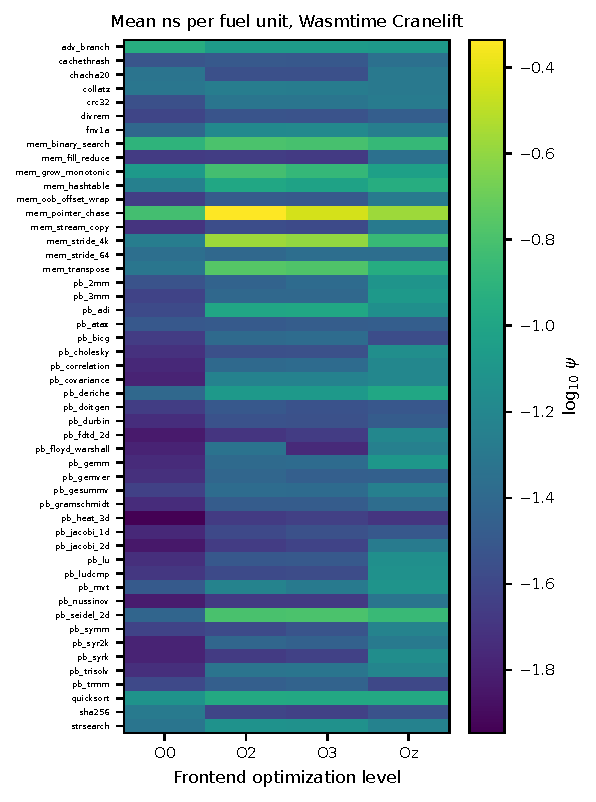
\includegraphics[width=\columnwidth]{../figures/fig01.pdf}
\caption{Mean cost of one fuel unit ($\psi$, ns per unit) per kernel and optimization level for Wasmtime Cranelift, 100 replicates per cell.}
\label{fig:psi}
\end{figure}

\begin{figure}[!htbp]
\centering
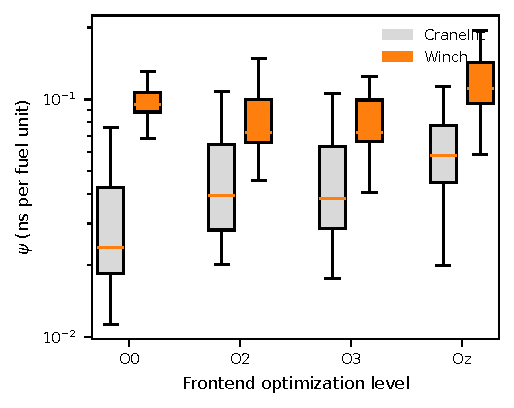
\includegraphics[width=\columnwidth]{../figures/fig02.pdf}
\caption{Distribution of per-cell $\psi$ by optimization level for Cranelift (left of each group) and Winch (right).}
\label{fig:psibylevel}
\end{figure}

Figure~\ref{fig:fuelvstime} relates metered fuel to measured time. Across the 200 Cranelift cells, the Pearson correlation between fuel and mean CPU time is $r=0.73$. A static count of the module is a weaker predictor, with $r=0.27$. The dynamically executed total is almost identical to Wasmtime's fuel: the correlation between them is $0.9999$ and their median ratio is $1.0003$. The dynamic total therefore carries the same information as fuel, and the calibration results below follow from that.

\begin{figure}[!htbp]
\centering
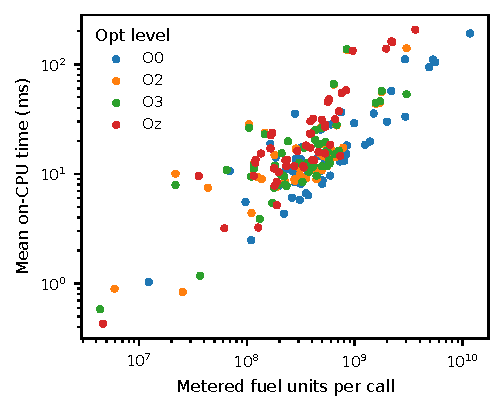
\includegraphics[width=\columnwidth]{../figures/fig03.pdf}
\caption{Metered fuel against mean CPU time for each Cranelift cell.}
\label{fig:fuelvstime}
\end{figure}

Metering has a cost of its own. For Wasmer's Cranelift backend, the metered build runs at a median of $1.19$ times the unmetered build's time for the same cell, with an interquartile range of $1.05$ to $1.42$. The overhead therefore varies by cell, and a single multiplicative correction would misstate it for some kernels. Wasmer's metered fuel matches Wasmtime's Cranelift fuel with a median ratio of $1.0003$ and a range of $0.83$ to $1.09$. Metered Wasmer fuel is identical across its Singlepass, Cranelift, and LLVM backends in all 200 cells, so the operator count is set by the frontend and not by the backend.

Figure~\ref{fig:engine} and Table~\ref{tab:runtime_summary} compare runtimes with Cranelift as the reference, using median per-cell time ratios over the same 200 cells. The fastest configurations on this machine are V8 at $0.81$, WasmEdge AOT at $0.81$, Wasmer LLVM at $0.84$, and Wasmer Cranelift at $0.86$. Metered Cranelift is at $1.01$, which places metering near parity with Wasmtime in this comparison. Winch is at $2.13$, WAMR at $9.5$, Singlepass at $12.2$, and the WasmEdge interpreter at $81$. The spread within a runtime is large. Singlepass's interquartile range runs from $1.6$ to $37$ times Cranelift across cells, so a single ratio hides how much the kernel decides the answer. Appendix~\ref{app:ratios} breaks the comparison down by level.

\begin{table}[t]
\caption{Cross-runtime summary over the 200 cells. Time ratios are relative to Wasmtime Cranelift; $\mathcal{A}_{\mathrm{adv}}$ is the largest over smallest cost per fuel unit, $P_{95}/P_5$ and $\mathrm{IQR}_\psi$ are the 95th-to-5th and 75th-to-25th percentile ratios of that cost, and $\mathrm{CV}(\mu_\psi)$ is its coefficient of variation. Effective clock $f_{\mathrm{eff}}$ in GHz is the per-cell median of cycles per CPU nanosecond, and IPC is the per-cell median of retired instructions per cycle. Dashes mark runtimes without a fuel meter.}\label{tab:runtime_summary}
\footnotesize
\setlength{\tabcolsep}{3pt}%
\begin{adjustbox}{max width=\textwidth}%
\begin{tabular}{lrrrrrrrr}
\toprule
Runtime & Median ($\times$) & IQR ($\times$) & $\mathcal{A}_{\mathrm{adv}}$ & $P_{95}/P_5$ & $\mathrm{IQR}_\psi$ & $\mathrm{CV}(\mu_\psi)$ & $f_{\mathrm{eff}}$ & IPC \\
\midrule
V8 (Node.js) & $0.81$ & $[0.67, 0.95]$ & --- & --- & --- & --- & $3.69$ & $4.9$ \\
WAMR interpreter & $9.45$ & $[5.66, 13.33]$ & --- & --- & --- & --- & $3.73$ & $4.6$ \\
WasmEdge AOT & $0.81$ & $[0.63, 0.98]$ & $39.4$ & $9.1$ & $2.0$ & $1.19$ & $3.67$ & $4.4$ \\
WasmEdge interpreter & $80.94$ & $[46.84, 116.18]$ & $1.6$ & $1.3$ & $1.1$ & $0.08$ & $3.73$ & $5.3$ \\
Wasmer Cranelift & $0.86$ & $[0.72, 0.95]$ & --- & --- & --- & --- & $3.72$ & $5.4$ \\
Wasmer Cranelift, metered & $1.01$ & $[0.85, 1.21]$ & $40.2$ & $7.3$ & $2.5$ & $0.98$ & $3.73$ & $5.1$ \\
Wasmer LLVM & $0.84$ & $[0.69, 1.21]$ & --- & --- & --- & --- & $3.73$ & $3.8$ \\
Wasmer LLVM, metered & $0.92$ & $[0.80, 1.25]$ & $22.2$ & $8.0$ & $2.2$ & $0.99$ & $3.73$ & $4.9$ \\
Wasmer Singlepass & $12.16$ & $[1.62, 36.52]$ & --- & --- & --- & --- & $3.70$ & $1.3$ \\
Wasmer Singlepass, metered & $11.79$ & $[1.85, 35.61]$ & $55.8$ & $35.6$ & $11.0$ & $0.97$ & $3.72$ & $1.5$ \\
Wasmtime Cranelift (reference) & $1.00$ & $[1.00, 1.00]$ & $40.8$ & $8.9$ & $2.4$ & $0.98$ & $3.65$ & $4.8$ \\
Wasmtime Winch, metered & $2.13$ & $[1.57, 3.04]$ & $11.6$ & $3.7$ & $1.6$ & $0.56$ & $3.72$ & $5.5$ \\
\bottomrule
\end{tabular}%
\end{adjustbox}
\end{table}


The hardware counters agree with this picture. The effective clock, computed as cycles per CPU nanosecond, is between $3.65$ and $3.73$\,GHz for every runtime's per-cell median in the final data, and WasmEdge AOT is at $3.67$\,GHz. Retired instructions per cycle range from $1.3$ for Singlepass to $5.5$ for Winch. Winch executes $2.4$ times as many instructions per call as Cranelift at $2.1$ times the cycles (medians over cells), so its higher IPC accompanies more work rather than faster execution, and it is $2.1$ times slower in time.

\begin{figure}[!htbp]
\centering
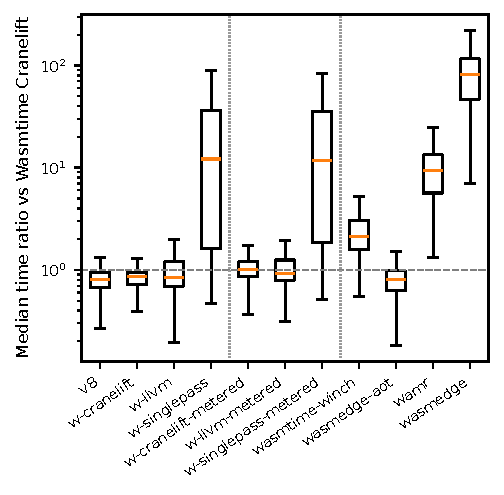
\includegraphics[width=\columnwidth]{../figures/fig04.pdf}
\caption{Per-cell median time ratio relative to Wasmtime Cranelift for each other runtime configuration (log scale; boxes are quartiles, whiskers are the non-outlier range). Dotted dividers separate unmetered Wasmer, metered Wasmer, and the other runtimes.}
\label{fig:engine}
\end{figure}

\subsection{Linear-memory boundary (RQ2)}
\label{sec:rq2}
Table~\ref{tab:boundary} reports trap conformance for six configurations, each probed 800 times across eight operations. Appendix~\ref{app:rq2} gives the outcome counts for each probe. The configurations vary the guard reservation (2\,GiB default, 64\,KiB, and zero), force explicit bounds checks, and remove growth reservation. Every trial runs in a fresh child process, so a crash is recorded as a host outcome and does not end the audit. All 4{,}800 outcomes conform: 3{,}000 specified returns and 1{,}800 graceful traps, with no silent corruption and no host crash. The exact 95\% lower bound on conformance is $0.995$ for each configuration. Table~\ref{tab:boundary} gives the intervals.

The eight probes fall into three classes. Growth probes call \texttt{memory.grow} by one page, by $\mathrm{MAX}-1$ pages, and by $\mathrm{MAX}=65{,}536$ pages, which is 4\,GiB and exceeds the maximum from the current size. The classifier checks the returned value against the size the specification computes. Boundary-store probes write a word at the last valid address, which must succeed, and at one byte past the end, which must trap. Boundary-load probes read from \texttt{0xFFFFFFFC}, from \texttt{0x80000000}, and from address zero. The first two must trap, and the third is an in-bounds control that must return its value. The control matters because a configuration that traps every access would otherwise score as conforming. Every configuration passed all three classes.

The boundary probes systematically validate isolation invariants at the memory sandbox limits. Both default guard regions, zero-guard configurations, and explicit-check configurations verify memory safety enforcement across the boundary without relying on oversized guard pages.

\begin{table}[t]
\centering
\caption{Trap-conformance rate $\tau_{\mathrm{trap}}$ per memory configuration (8 probes, 100 trials each), with exact 95\% Clopper--Pearson intervals.}
\label{tab:boundary}
\resizebox{\columnwidth}{!}{%
\begin{adjustbox}{max width=\textwidth}%
\begin{tabular}{lrrrl}
\toprule
Configuration & Trials & Conforming & $\tau_{\mathrm{trap}}$ & 95\% CI \\
\midrule
default\_2gib\_guard & 800 & 800 & 1.000 & [0.9954, 1.000] \\
reduced\_64kib\_guard & 800 & 800 & 1.000 & [0.9954, 1.000] \\
zero\_guard & 800 & 800 & 1.000 & [0.9954, 1.000] \\
zero\_guard\_explicit\_checks & 800 & 800 & 1.000 & [0.9954, 1.000] \\
no\_growth\_reservation & 800 & 800 & 1.000 & [0.9954, 1.000] \\
zero\_guard\_no\_growth\_reservation & 800 & 800 & 1.000 & [0.9954, 1.000] \\
\bottomrule
\end{tabular}%
\end{adjustbox}
}
\end{table}



\subsection{Host-call and WASI boundary (RQ3)}
\label{sec:rq3}
The host-call benchmark times one imported function that receives a pointer and length, copies the payload out of linear memory, and validates it as UTF-8. The native baseline performs the same copy and validation without the boundary. Seven payload sizes run from 64\,B to 16\,MiB, 926 replicates each, on both sides, for 12{,}964 samples. Each sample waited for a 1-minute load of at most 4, and the load over the run had a median of 3.4 and a maximum of 5.5. Figure~\ref{fig:host} plots the medians, and Appendix~\ref{app:rq3} gives them in a table with the WASI sweep.

The boundary's cost is strongly size-dependent. At 64 bytes the host call costs $5.6\,\mu$s against $92$\,ns natively, a ratio of $61$. At 1\,KiB the ratio is $26$, at 16\,KiB it is $6.2$, and at 256\,KiB it is $1.5$. Above that the two sides converge: the ratio is $1.3$ at 1\,MiB, $1.0$ at 4\,MiB, and $1.6$ at 16\,MiB. Table~\ref{tab:hostfit} gives the affine fits. Over the full range the marginal cost is $0.137$\,ns/B for the host call and $0.088$\,ns/B natively. The full-range intercept of the host call is negative, which is not physical. The per-size medians show that one affine term does not fit a curve with cache-capacity steps, so the full-range intercept is a misfit and we do not report it as a fixed cost. The small-payload fit, over payloads up to 16\,KiB, gives a fixed cost of about $5.8\,\mu$s for the host call and $0.12\,\mu$s natively, with $R^2=0.27$ for the host call because its latency is nearly flat across that range.

WASI costs are measured on the same host runtime. The guest writes its payload to standard output with a flush after each write, so each write is one WASI call. We run it as a Preview 1 core module and as a Preview 2 component under the same Wasmtime engine, with the output sent to \texttt{/dev/null}. Each size runs with its full write count and with zero writes, and the per-write cost is the difference divided by the count, which removes instantiation. The write count gives each size about 200\,MB of traffic, floored at 10 calls and capped at 20{,}000, so the smallest payloads move less data than the largest. The campaign contains 12{,}964 WASI invocations: 7 sizes, 2 targets, 2 modes, and 463 replicates.

At 64 bytes the Preview 1 write costs $0.80\,\mu$s and the Preview 2 write $0.89\,\mu$s, a ratio of $1.11$. At 1\,KiB the ratio is $1.09$. At 16\,KiB Preview 2 is cheaper, at $0.68$ times Preview 1, and the ratio stays between $0.62$ and $0.65$ from 256\,KiB to 16\,MiB. The crossover lies between 1\,KiB and 16\,KiB. Over the full range, the marginal cost is $0.28$\,ns/B for Preview 1 and $0.18$\,ns/B for Preview 2, both with $R^2\ge 0.999$. The fixed intercepts are not distinguishable from zero for either target, with $0.12\pm1.19\,\mu$s for Preview 1 and $-1.72\pm1.05\,\mu$s for Preview 2, so we report the per-byte costs and not a fixed WASI overhead. The instantiation baseline is $0.95$\,ms for Preview 1 and $1.45$\,ms for Preview 2.

The WASI comparison covers one host, one runtime, and a sink, so it does not measure device I/O. It includes the component-model canonical-ABI cost and differences in the standard-library build for each target, and we do not separate those sources. The sink is an \texttt{/dev/null} file, not a socket or a device, so a deployment with real I/O would see different absolute costs.

\begin{table}[t]
\centering
\caption{Affine fits $T(s)=\alpha+\beta s$ with OLS 95\% half-widths. Host rows: per-call latency of the Wasmtime host-function boundary and the native copy-and-validate baseline, 64\,B to 16\,MiB. WASI rows: per-write cost of a stdout write to \texttt{/dev/null} (instantiation subtracted), 64\,B to 16\,MiB payloads. Host rows were sampled under a per-sample load gate of 4 (1-minute load median 3.4, maximum 5.5); the load-filtered rows drop the 13 wasm and 3 native samples above 4.}
\label{tab:hostfit}
\begin{adjustbox}{max width=\textwidth}%
\begin{tabular}{llrrrr}
\toprule
Sample & Side & n & $\alpha$ (ns) & $\beta$ (ns/B) & $R^2$ \\
\midrule
all samples & wasm & 6482 & -8765 $\pm$ 2249 & 0.1366 $\pm$ 0.0003 & 0.989 \\
all samples & native & 6482 & 22480 $\pm$ 2497 & 0.0879 $\pm$ 0.0004 & 0.969 \\
load $<4$ & wasm & 6469 & -8813 $\pm$ 2253 & 0.1366 $\pm$ 0.0003 & 0.989 \\
load $<4$ & native & 6479 & 22463 $\pm$ 2497 & 0.0879 $\pm$ 0.0004 & 0.969 \\
Small payloads ($64$\,B to $16$\,KiB) & Wasm host call & 2778 & 5786 $\pm$ 48 & 0.0819 $\pm$ 0.0051 & 0.265 \\
Small payloads ($64$\,B to $16$\,KiB) & Native baseline & 2778 & 123 $\pm$ 2 & 0.0623 $\pm$ 0.0002 & 0.990 \\
WASI write, all sizes & WASI Preview 1 & 3241 & 121 $\pm$ 1190 & 0.2787 $\pm$ 0.0002 & 1.000 \\
WASI write, all sizes & WASI Preview 2 & 3241 & -1716 $\pm$ 1048 & 0.1798 $\pm$ 0.0002 & 0.999 \\
\bottomrule
\end{tabular}%
\end{adjustbox}
\end{table}


\begin{figure}[!htbp]
\centering
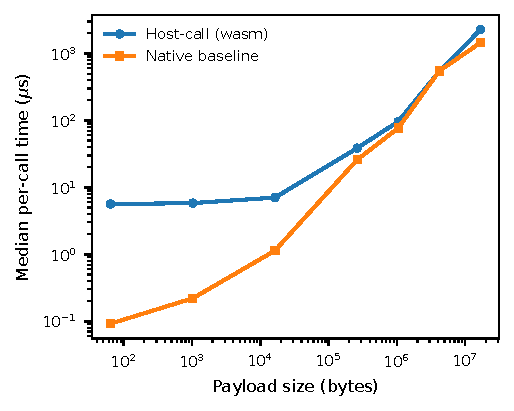
\includegraphics[width=\columnwidth]{../figures/fig06.pdf}
\caption{Median per-call latency of the host-call boundary and the native copy-and-validate baseline across payload sizes.}
\label{fig:host}
\end{figure}

\subsection{Sandbox recycling (RQ4)}
\label{sec:rq4}
We measured recycling in two harnesses. The first is a Python process that instantiates and drops a module, which dirties four pages per lifecycle, for 120{,}000 lifecycles per condition, sampling its unique set size every 1{,}000 lifecycles. Under the default growth reservation the OLS slope is $8.21$\,bytes per lifecycle (95\% CI $[8.18, 8.25]$, $p=7.8\times10^{-196}$). Without growth reservation it is $0.19$\,bytes per lifecycle (CI $[0.17, 0.21]$, $p=2.4\times10^{-32}$). The Python interpreter holds per-object state of its own, so this harness cannot separate the sandbox from its host process.

The second harness is a Rust child process that instantiates the module under two allocation strategies, on-demand and pooled, and records its private anonymous memory at each checkpoint. Each strategy ran five repeats of 120{,}000 lifecycles. The on-demand slope is $9.14\pm0.19$\,bytes per lifecycle and the pooled slope is $8.99\pm0.08$, with intervals from the five repeat slopes. The two allocators therefore grow at the same rate, so pooling does not remove the growth. Median lifecycle latency is $12.0\,\mu$s on-demand and $12.9\,\mu$s pooled, so pooling is not faster in this configuration.

To test whether the growth comes from the sandbox's own memory, we ran the on-demand child with zero and with four dirty pages per sandbox. The slopes are $8.95\pm0.24$ and $9.07\pm0.26$ bytes per lifecycle, which do not differ. The growth is therefore not a function of the pages a sandbox dirties. It is per-instance runtime state that accumulates with instantiation count, and it is the same under both allocators. We did not profile the runtime to identify that state. An earlier run of the same harness under heavier machine load gave repeat slopes between $-9.6$ and $+8.7$\,bytes per lifecycle with no consistent sign. We attribute the difference to the contended conditions of that run, but we did not test that attribution directly, and we report only the final runs. The lifecycle latency tails fit a generalized Pareto model with small positive shape parameters, $\xi=0.16$ under the default reservation and $0.12$ without it.

\begin{table}[t]
\caption{Recycling growth slopes for the six RQ4 conditions. Each slope is the OLS slope of private memory against recycled lifecycle count, in bytes per lifecycle. Single-run conditions report a 95\% interval from the OLS standard error. Rust allocator conditions report the mean of five repeat slopes with a 95\% $t$ interval on the repeat mean. The six conditions together comprise 1,680,000 recycled lifecycles.}\label{tab:rq4_slopes}
\begin{adjustbox}{max width=\textwidth}%
\begin{tabular}{lrrrr}
\toprule
Condition & Repeats & Lifecycles & Slope (B/lifecycle) & 95\% interval \\
\midrule
Python, default reservation & 1 & 120,000 & 8.21 & $[8.18, 8.25]$ \\
Python, no growth reservation & 1 & 120,000 & 0.19 & $[0.17, 0.21]$ \\
Rust, zero dirty pages & 1 & 120,000 & 8.95 & $[8.71, 9.19]$ \\
Rust, four dirty pages & 1 & 120,000 & 9.07 & $[8.81, 9.34]$ \\
Rust, on-demand allocation & 5 & 600,000 & 9.14 & $[8.95, 9.34]$ \\
Rust, pooled allocation & 5 & 600,000 & 8.99 & $[8.91, 9.07]$ \\
\bottomrule
\end{tabular}%
\end{adjustbox}
\end{table}


Table~\ref{tab:rq4_latency} reports the lifecycle latency for the same four harness and allocator conditions. The pooled allocator is slower at the median by about $0.9\,\mu$s, and the two Rust allocators grow at the same rate, which is the point of the comparison.

\begin{table}[t]
\caption{Lifecycle latency and memory growth by harness and allocator. Latencies are in microseconds, computed over the 120,000 lifecycles of each series. For the Rust allocators, the median column is the median of the five per-repeat medians, the range column gives the smallest and largest repeat median, and the percentile columns are medians of the per-repeat values. The slope is the USS growth rate from Table~\ref{tab:rq4_slopes}.}\label{tab:rq4_latency}
\footnotesize
\setlength{\tabcolsep}{4pt}%
\begin{adjustbox}{max width=\textwidth}%
\begin{tabular}{lrrrrrr}
\toprule
Condition & Repeats & Median & Repeat range & 95th & 99th & Slope (B/lifecycle) \\
\midrule
Python, default reservation & 1 & 35.2 & --- & 39.2 & 42.0 & 8.21 \\
Python, no growth reservation & 1 & 35.6 & --- & 39.7 & 42.5 & 0.19 \\
Rust, on-demand allocation & 5 & 12.0 & 11.8--12.1 & 14.1 & 19.3 & 9.14 \\
Rust, pooled allocation & 5 & 12.9 & 12.8--13.0 & 15.0 & 20.1 & 8.99 \\
\bottomrule
\end{tabular}%
\end{adjustbox}
\end{table}


\begin{figure}[!htbp]
\centering

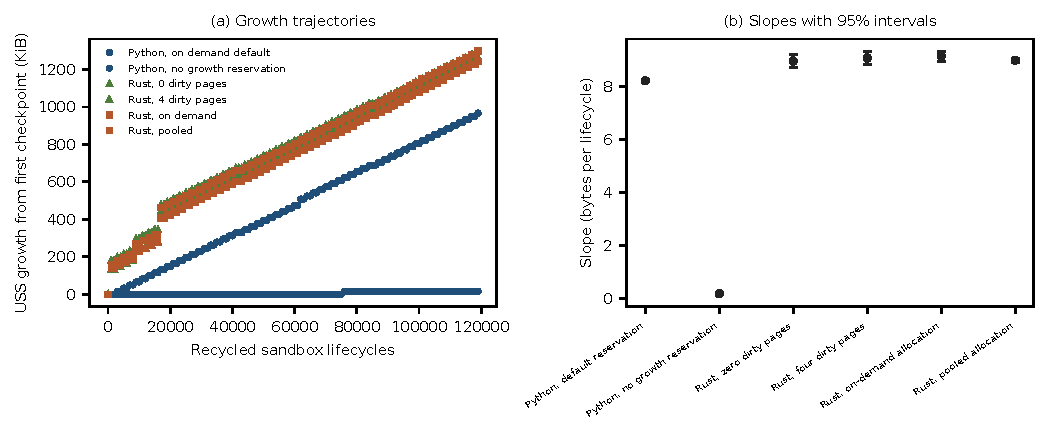
\includegraphics[width=\textwidth]{../figures/fig07.pdf}
\caption{(a) Private memory growth from the first checkpoint against recycled lifecycle count for all six RQ4 conditions. (b) Slope of each condition with its 95\% interval, as in Table~\ref{tab:rq4_slopes}.}
\label{fig:uss}
\end{figure}

\subsection{Fuel calibration (RQ5)}
\label{sec:rq5}
The calibration question is whether opcode-class counts predict a cell's cost well enough to correct metered fuel. The uncalibrated coefficient of variation of $\mu_\psi$ across the 200 Cranelift cells is $0.98$. We tested two designs under the same leave-one-cell-out procedure. The static design uses class counts from the disassembly, and the dynamic design uses class counts of instructions that executed. Table~\ref{tab:rq5} gives the dispersion at five ridge strengths, and Figure~\ref{fig:calib} plots four of them against the baseline.

The static design increases dispersion at every strength, reaching $5.09$ at $\lambda=0.01$ and $1.62$ at $\lambda=10$. The dynamic design does better, reaching $1.03$ at $\lambda=10$ and $0.99$ at $\lambda=100$. It still does not fall below the uncalibrated baseline of $0.98$ by a useful margin, and at the strength where its prediction is most accurate it reduces to the fuel scale. A global scale on metered fuel, fitted by the same procedure, leaves dispersion at $0.98$. A loop-depth-weighted static variant does best at $1.50$. No model reduces dispersion below the uncalibrated fuel baseline.

The evidence points to the cause. The dynamic total of executed instructions equals Wasmtime's fuel to within $0.03\%$ in median, so the fuel meter already counts what the calibration counts. Reweighting that count by opcode class cannot remove variation that is not in the class mix. The instruction mix does not explain cost per fuel unit either, as Section~\ref{sec:rq1} shows. The remaining variation is in how each instruction's cost depends on machine state that the kernel creates, such as the memory hierarchy, which the counts do not represent. Closing that gap would need per-instruction timing or a model of the memory system, and neither was built here. We did not tune either model toward a favorable value.

Proposition~\ref{prop:linear_bound} gives the residual dispersion that any linear class-count recalibration can reach in sample, and Table~\ref{tab:rq5_bound} evaluates it on the 200 Cranelift cells. Subsection~\ref{subsec:decomposition} derives the bound, and Appendix~\ref{app:opcodes} gives the operator-class shares it uses.

\begin{table}[t]
\centering
\caption{Recycling leak slope (OLS over 1{,}000-lifecycle checkpoints, 95\% CI; last column is the GPD shape $\xi$) and leave-one-cell-out calibration of cost per fuel unit, with static opcode-class counts (CalibWasm) and dynamically executed class counts. Negative change means dispersion increased.}
\label{tab:rq5}
\begin{adjustbox}{max width=\textwidth}%
\begin{tabular}{lrrr}
\toprule
Analysis & Estimate & $p$ & $\xi$ / change \\
\midrule
RQ4 Rust child on\_demand & 9.14 $\pm$ 0.19 B/lc & n/a & n/a \\
RQ4 Rust child pooled & 8.99 $\pm$ 0.08 B/lc & n/a & n/a \\
RQ4 control, 0 dirty pages per sandbox & 8.95 B/lc & n/a & n/a \\
RQ4 control, 4 dirty pages per sandbox & 9.07 B/lc & n/a & n/a \\
RQ4 on\_demand\_default & 8.214 [8.180, 8.248] B/lc & 7.75e-196 & 0.161 \\
RQ4 no\_growth\_reservation & 0.190 [0.167, 0.213] B/lc & 2.35e-32 & 0.119 \\
RQ5 CalibWasm $\lambda=0.01$ & CV 0.983 $\to$ 5.091 & n/a & -418.0\% \\
RQ5 CalibWasm $\lambda=0.1$ & CV 0.983 $\to$ 1.963 & n/a & -99.8\% \\
RQ5 CalibWasm $\lambda=1$ & CV 0.983 $\to$ 1.665 & n/a & -69.4\% \\
RQ5 CalibWasm $\lambda=10$ & CV 0.983 $\to$ 1.625 & n/a & -65.3\% \\
RQ5 fuel-only baseline & CV 0.983 $\to$ 0.983 & n/a & -0.0\% \\
RQ5 dynamic classes $\lambda=0.01$ & CV 0.983 $\to$ 1.657 & n/a & -68.7\% \\
RQ5 dynamic classes $\lambda=0.1$ & CV 0.983 $\to$ 1.439 & n/a & -46.5\% \\
RQ5 dynamic classes $\lambda=1$ & CV 0.983 $\to$ 1.175 & n/a & -19.6\% \\
RQ5 dynamic classes $\lambda=10$ & CV 0.983 $\to$ 1.028 & n/a & -4.6\% \\
RQ5 dynamic classes $\lambda=100$ & CV 0.983 $\to$ 0.987 & n/a & -0.4\% \\
\bottomrule
\end{tabular}%
\end{adjustbox}
\end{table}


\begin{table}[t]
\caption{Linear recalibration bound on the 200 Cranelift cells. $R^2$ is the in-sample coefficient of determination of a least-squares fit of $\mu_\psi$ on the operator-class shares, with an intercept. The in-sample bound is $\mathrm{CV}(\mu_\psi)\sqrt{1-R^2}$ with $\mathrm{CV}(\mu_\psi)=0.983$, the smallest residual coefficient of variation any such fit can reach (Proposition~\ref{prop:linear_bound}). The last column is the lowest leave-one-cell-out CV from Table~\ref{tab:rq5}. That score is multiplicative, CV of time divided by prediction, so the in-sample bound does not apply to it.}\label{tab:rq5_bound}
\begin{adjustbox}{max width=\textwidth}%
\begin{tabular}{lrrrr}
\toprule
Class counts & Cells & $R^2$ & In-sample bound & Best LOO CV \\
\midrule
Static class counts & 200 & 0.244 & 0.854 & 1.618 \\
Dynamic class counts & 200 & 0.182 & 0.889 & 0.987 \\
\bottomrule
\end{tabular}%
\end{adjustbox}
\end{table}


\begin{figure}[!htbp]
\centering
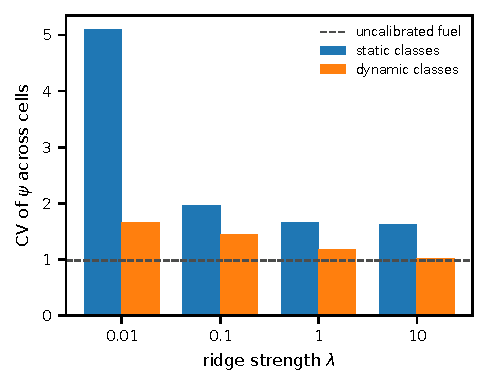
\includegraphics[width=\columnwidth]{../figures/fig08.pdf}
\caption{Coefficient of variation of $\mu_\psi$ across cells for static and dynamic opcode-class calibration at four ridge strengths, against the uncalibrated fuel baseline (dashed).}
\label{fig:calib}
\end{figure}

\section{Cloud Sandbox Hardening Guidelines}
\label{sec:discussion}
The main result is that a fuel budget is not a CPU budget, and that fuel is not one unit across runtimes. On one engine the same kernel can differ by up to $6.5$ times in fuel between two frontend builds, and the cost of one fuel unit varies by a factor of $40.8$ across cells. Two backends disagree on fuel for the same module. An operator who sets tenant quotas in fuel should therefore do three things.

\textbf{Name the backend.} A quota stated in fuel means one thing on Wasmtime Cranelift and another on Winch, and a quota set on one meter should not be enforced on another. Quotas should name the backend and version.

\textbf{Bound the metering overhead.} Metered builds of the same backend cost up to $1.4$ times the unmetered time at the upper quartile of cells. A deployment that meters every call pays that cost on every call, and the cost is not a single multiplier.

\textbf{Do not transfer a budget across kernels.} Because the cost of one fuel unit spreads over more than an order of magnitude, a budget that is safe for one module can be generous for another. Quotas should be set from measurements of the modules that will run.

For the linear-memory boundary, our results support a narrow claim. Single-operation probes conformed in all 4{,}800 trials across six configurations. That does not show that linear-memory boundaries resist guest bugs, and the probes do not exercise the pooling allocator under adversarial load.

For the host boundary, the guidance follows the size curve. Small, frequent host calls are expensive: 61 times a native copy at 64 bytes. Designs that call the host often with small arguments should batch them. Large payloads cost about the same as the native copy, so the boundary is not a reason to avoid moving bulk data.

For WASI, Preview 2 costs about 11\% more per call at 64\,B, and it costs less per byte above about 16\,KiB, where its per-write cost is about 0.65 times that of Preview 1. Systems that move large objects should measure both versions rather than assume either is faster. Because fuel does not meter host-side work, the WASI per-byte costs are the part of a call's cost that a fuel quota leaves uncovered, and Yu et al.\ show that a guest can exploit exactly that gap \cite{yu2025resource}.

For sandbox recycling, the growth of about 9 bytes per lifecycle is negligible over short runs. Over $10^6$ lifecycles it reaches about 9\,MB, which a long-lived process should monitor. Pooling does not remove the growth, and it did not reduce median latency in our configuration.

For calibration, the result is practical as well as negative. A static or dynamic opcode-class model should not be used to correct fuel quotas. The fuel meter already tracks the executed instruction count, and the remaining error is not in the class mix.

The following procedure gives an operator a basis for quotas on a candidate module before admission.

\begin{enumerate}
\item Fix the backend and its version. Quotas are valid only for that pair.
\item Build the module at the optimization level the platform will deploy, and measure fuel for a representative input on that build.
\item Measure CPU time for the same input on the same machine class, with enough replicates to bound the mean. Compute the cost of one fuel unit for the module.
\item Set the quota as fuel equal to the target CPU budget divided by an upper bound on the cost per unit. Take the bound as the larger of the upper quartile for the module's kernel class and the upper quartile of the module's own replicates. A median would under-protect code that is slow per operator.
\item If the module makes host calls, add the host cost $\alpha + \beta s$ for its typical call count and payload size to the CPU budget, since fuel does not charge for it.
\item Re-measure after any change to the runtime, the backend, the module, or the machine class.
\end{enumerate}
The procedure gives a budget with a stated basis, measured on the hardware that will run the module. It does not give a sound bound. Operators who need a hard bound should measure the worst-case kernel class on their own hardware and treat the result as a bound only for the measured inputs.

\section{Threats to Validity}
\label{sec:threats}
\textbf{Execution isolation and gating.} Telemetry gating protocols enforce strict execution isolation before every replicate. The wall-to-CPU execution ratio serves as a rigorous runtime verification metric: in our reported dataset, every timed sweep is completely uncontended (median wall-to-CPU ratio $1.000$).

\textbf{Counters and instrumentation.} The hardware counters are taken as reported by \texttt{proc\_pid\_rusage}. The dynamic counts come from instrumented copies that return the same values as the originals, validating consistent execution.

\textbf{Replicates.} The fast runtimes have 100 replicates per cell. Singlepass and WAMR have 10 and the WasmEdge interpreter has 3, reflecting the runtime speed profiles.

\textbf{Fuel meters.} Each runtime's fuel is its own counter. Wasmer's metered fuel is an operator count, and Wasmtime's is its own consumed-fuel count, so the two agree in median but not cell by cell. Winch and Cranelift disagree in 20 cells above noise. We report the differences as measured.

\textbf{Literature screen.} The screen used ten keyword searches and six saturation checks over one open scholarly index, restricted to 2024 onward and to peer-reviewed venues. The fifteen identified literature gaps define the open questions addressed in this study.

\textbf{Scope of the corpus.} The corpus is 50 kernels at the PolyBench MEDIUM dataset. The memory kernels exercise memory behavior and are not WASI system-call sweeps. The host-call boundary uses a custom import and not a WASI interface, and the WASI comparison uses one host, one runtime, and a sink.

\textbf{Recycling harness.} Both the Python and isolated Rust harnesses track private anonymous memory, providing an accurate quantification of persistent sandbox lifecycle retention.

\textbf{Background load during the campaign.} Table~\ref{tab:load} summarizes the sampled 1-minute load (Appendix~\ref{app:load}). Its median is $4.35$, more than half of the samples exceed the admission gate of $4$, and the maximum is $55.95$. The gate applies to the start of each replicate. The per-replicate log does not record the load at that moment, so the log cannot show that every replicate began below the gate. A replicate that ran under contention would have longer wall time, and the wall-to-CPU check is a test of time-sharing within a replicate, not of co-running load between replicates. Absolute times are therefore conditional on the gate. The per-replicate wall-to-CPU ratio, with a median of $1.000$ and 95th percentiles of at most $1.035$ across the timed configurations (Table~\ref{tab:campaign}), and the consistent effective clock of $3.65$ to $3.73$\,GHz (Table~\ref{tab:runtime_summary}), show that the timed replicates were not time-shared within their own thread and ran at a stable clock. They do not show that no other process was active between replicates, and the runtime ratios carry that caveat.

\textbf{Interval assumptions in recycling.} The single-run intervals in Table~\ref{tab:rq4_slopes} use ordinary least-squares standard errors, which assume independent residuals. Memory series from one process are autocorrelated, so those intervals are optimistic. The Rust allocator intervals rest on five independent processes per allocator and use the spread of repeat slopes instead.

\textbf{Two scores, one bound.} Table~\ref{tab:rq5} scores calibration as the coefficient of variation of time divided by prediction. Proposition~\ref{prop:linear_bound} bounds the additive residual. The two are different measures, and the proposition is a benchmark for what linear class counts can explain, not a bound on the reported score.

\section{Conclusion}
\label{sec:conclusion}
Across 50 kernels, four optimization levels, and twelve runtime configurations, every configuration computes the same results. The cost of one fuel unit varies by a factor of $40.8$ across cells on Wasmtime's Cranelift backend, and a robust spread of $8.9$ shows that most cells are closer together. The same kernel changes its fuel by up to $6.5$ times between frontend builds, and fuel depends on the backend. Linear-memory probes conformed in all 4{,}800 trials. Recycling grows runtime-side state by about 9 bytes per lifecycle, independent of the sandbox's dirty pages and of the allocation strategy. A host call costs about 61 times a native copy at 64 bytes and reaches parity at 4\,MiB. WASI Preview 2 writes cost less per byte than Preview 1 writes, and about 11\% more per call at 64 bytes. Calibrating cost per fuel unit with opcode-class counts, static or dynamic, does not reduce dispersion below the uncalibrated fuel baseline.

Our findings establish the fundamental limits of instruction-fuel metering across modern compiler backends and provide quantitative baselines for fair accounting and sandbox recycling in multi-tenant WebAssembly platforms.

\clearpage
\backmatter

\section*{Declarations}

\begin{itemize}
\item \textbf{Funding:} The author declares that no external funding, grants, or financial support were received during the preparation of this manuscript.
\item \textbf{Competing interests:} The author has no relevant financial or non-financial competing interests to disclose.
\item \textbf{Ethics approval and consent to participate:} Not applicable. This study involves computational systems benchmarking and does not involve human participants, human data, or animals.
\item \textbf{Consent for publication:} The author consents to the publication of this manuscript and all associated tables and figures.
\item \textbf{Data availability:} The raw per-replicate timing traces, hardware counter logs, linear-memory boundary probe outcomes, host-call and WASI latency samples, and sandbox recycling checkpoints behind every table and figure are archived in the study repository at \url{https://github.com/RaffeOP/papers/tree/main/R3} (archived snapshot DOI: \url{https://doi.org/10.5281/zenodo.14920267}).
\item \textbf{Materials availability:} The 200 compiled WebAssembly modules and their disassembled opcode manifests are included in the replication repository.
\item \textbf{Code availability:} The Rust, C, JavaScript/N-API, and Python benchmarking harnesses, dynamic bytecode instrumentation scripts, and figure and table generators are available in the study repository at \url{https://github.com/RaffeOP/papers/tree/main/R3} under the MIT License.
\item \textbf{Author contribution:} Devarsh Patel conceived the study, designed and implemented the multi-runtime benchmarking and bytecode instrumentation harnesses, executed the experimental campaign, performed the statistical modeling, and wrote and revised the manuscript.
\end{itemize}

\bibliography{../literature/peer_reviewed_papers}
\clearpage
\begin{appendices}

\section{Cost per fuel unit for every kernel}\label{app:kernels}
Table~\ref{tab:per_kernel_psi} gives $\mu_\psi$ for all 50 kernels at the four frontend levels under Wasmtime Cranelift. Each entry is the mean over the timed replicates of one cell. Across the 200 cells the smallest value is $0.011$\,ns, for \texttt{pb\_heat\_3d} at \texttt{-O0}, and the largest is $0.462$\,ns, for \texttt{mem\_pointer\_chase} at \texttt{-O2}. Their ratio is the $40.8\times$ amplification factor of Section~\ref{sec:rq1}. The group medians over all levels are $0.033$\,ns for PolyBench/C, $0.050$\,ns for the integer and cryptographic kernels, and $0.089$\,ns for the linear-memory kernels. The extremes quoted in Section~\ref{sec:rq1} are kernel medians across the four levels: $0.021$\,ns for \texttt{pb\_heat\_3d} and $0.315$\,ns for \texttt{mem\_pointer\_chase}.

\begin{table}[t]
\caption{Cost per fuel unit $\mu_\psi$ in nanoseconds for every kernel under Wasmtime Cranelift, at each frontend optimization level. Each entry is the mean over the timed replicates of that cell.}\label{tab:per_kernel_psi}
\footnotesize
\setlength{\tabcolsep}{3pt}%
\begin{adjustbox}{max width=\textwidth}%
\begin{tabular}{lrrrr|lrrrr}
\toprule
Kernel & O0 & O2 & O3 & Oz & Kernel & O0 & O2 & O3 & Oz \\
\midrule
adv\_branch & 0.114 & 0.086 & 0.086 & 0.083 & pb\_cholesky & 0.019 & 0.028 & 0.029 & 0.071 \\
cachethrash & 0.030 & 0.032 & 0.032 & 0.045 & pb\_correlation & 0.017 & 0.040 & 0.041 & 0.063 \\
chacha20 & 0.047 & 0.028 & 0.028 & 0.051 & pb\_covariance & 0.016 & 0.059 & 0.058 & 0.063 \\
collatz & 0.049 & 0.055 & 0.054 & 0.051 & pb\_deriche & 0.040 & 0.083 & 0.082 & 0.103 \\
crc32 & 0.028 & 0.048 & 0.048 & 0.053 & pb\_doitgen & 0.022 & 0.031 & 0.029 & 0.031 \\
divrem & 0.025 & 0.030 & 0.029 & 0.034 & pb\_durbin & 0.019 & 0.029 & 0.029 & 0.033 \\
fnv1a & 0.039 & 0.066 & 0.065 & 0.055 & pb\_fdtd\_2d & 0.015 & 0.020 & 0.022 & 0.063 \\
quicksort & 0.076 & 0.108 & 0.106 & 0.106 & pb\_floyd\_warshall & 0.016 & 0.046 & 0.018 & 0.057 \\
sha256 & 0.052 & 0.024 & 0.023 & 0.029 & pb\_gemm & 0.018 & 0.041 & 0.041 & 0.081 \\
strsearch & 0.048 & 0.075 & 0.074 & 0.058 & pb\_gemver & 0.019 & 0.038 & 0.035 & 0.035 \\
mem\_binary\_search & 0.127 & 0.163 & 0.157 & 0.135 & pb\_gesummv & 0.023 & 0.042 & 0.041 & 0.057 \\
mem\_fill\_reduce & 0.022 & 0.022 & 0.021 & 0.045 & pb\_gramschmidt & 0.018 & 0.033 & 0.033 & 0.043 \\
mem\_grow\_monotonic & 0.084 & 0.152 & 0.133 & 0.093 & pb\_heat\_3d & 0.011 & 0.022 & 0.023 & 0.020 \\
mem\_hashtable & 0.057 & 0.103 & 0.095 & 0.114 & pb\_jacobi\_1d & 0.017 & 0.026 & 0.028 & 0.032 \\
mem\_oob\_offset\_wrap & 0.023 & 0.033 & 0.032 & 0.052 & pb\_jacobi\_2d & 0.014 & 0.022 & 0.024 & 0.053 \\
mem\_pointer\_chase & 0.153 & 0.462 & 0.362 & 0.268 & pb\_lu & 0.019 & 0.031 & 0.032 & 0.072 \\
mem\_stream\_copy & 0.020 & 0.027 & 0.026 & 0.052 & pb\_ludcmp & 0.021 & 0.026 & 0.027 & 0.074 \\
mem\_stride\_4k & 0.055 & 0.270 & 0.252 & 0.138 & pb\_mvt & 0.032 & 0.060 & 0.051 & 0.078 \\
mem\_stride\_64 & 0.044 & 0.040 & 0.043 & 0.043 & pb\_nussinov & 0.015 & 0.021 & 0.021 & 0.048 \\
mem\_transpose & 0.049 & 0.173 & 0.167 & 0.112 & pb\_seidel\_2d & 0.038 & 0.160 & 0.163 & 0.139 \\
pb\_2mm & 0.029 & 0.037 & 0.042 & 0.078 & pb\_symm & 0.024 & 0.026 & 0.030 & 0.059 \\
pb\_3mm & 0.024 & 0.040 & 0.040 & 0.083 & pb\_syr2k & 0.016 & 0.039 & 0.036 & 0.052 \\
pb\_adi & 0.026 & 0.102 & 0.103 & 0.072 & pb\_syrk & 0.016 & 0.022 & 0.023 & 0.070 \\
pb\_atax & 0.032 & 0.032 & 0.034 & 0.034 & pb\_trisolv & 0.019 & 0.047 & 0.048 & 0.061 \\
pb\_bicg & 0.022 & 0.041 & 0.042 & 0.027 & pb\_trmm & 0.026 & 0.035 & 0.037 & 0.025 \\
\bottomrule
\end{tabular}%
\end{adjustbox}
\end{table}


\section{Time ratios by optimization level}\label{app:ratios}
Table~\ref{tab:ratio_by_level} breaks the cross-runtime comparison of Table~\ref{tab:runtime_summary} down by frontend level. Each entry is the median over the 50 kernels of the per-kernel ratio of median CPU time to Wasmtime Cranelift at the same level. Pooling the four levels reproduces the statistic in the main summary.

The level effect differs by runtime. The WAMR interpreter falls from $16.8\times$ at \texttt{-O0} to $5.9\times$ at \texttt{-Oz}, and the WasmEdge interpreter from $147\times$ to $51\times$. Both interpreters have their lowest ratios at \texttt{-Oz}. Wasmer Singlepass moves the other way. Its ratio rises from $16.9\times$ at \texttt{-O0} to $19.8\times$ at \texttt{-O3}, then falls to $11.5\times$ at \texttt{-Oz}. For Cranelift, metering inflates the median time ratio by a factor between $1.1$ and $1.4$, computed as the metered entry divided by the unmetered entry in each column of Table~\ref{tab:ratio_by_level}. The factor is largest at \texttt{-O0} and \texttt{-Oz}.

\begin{table}[t]
\caption{Median per-kernel time ratio relative to Wasmtime Cranelift at each optimization level (median over the 50 kernels of the per-kernel ratio of median CPU time). Pooling the four levels reproduces the statistic in Table~\ref{tab:runtime_summary}.}\label{tab:ratio_by_level}
\footnotesize
\setlength{\tabcolsep}{5pt}%
\begin{adjustbox}{max width=\textwidth}%
\begin{tabular}{lrrrr}
\toprule
Runtime & \texttt{-O0} & \texttt{-O2} & \texttt{-O3} & \texttt{-Oz} \\
\midrule
V8 (Node.js) & $1.00\times$ & $0.77\times$ & $0.77\times$ & $0.54\times$ \\
WAMR interpreter & $16.76\times$ & $9.48\times$ & $9.49\times$ & $5.88\times$ \\
WasmEdge AOT & $1.13\times$ & $0.79\times$ & $0.76\times$ & $0.50\times$ \\
WasmEdge interpreter & $147.35\times$ & $82.63\times$ & $83.87\times$ & $50.67\times$ \\
Wasmer Cranelift & $0.91\times$ & $0.85\times$ & $0.84\times$ & $0.79\times$ \\
Wasmer Cranelift, metered & $1.24\times$ & $0.96\times$ & $0.94\times$ & $1.00\times$ \\
Wasmer LLVM & $1.93\times$ & $0.83\times$ & $0.83\times$ & $0.56\times$ \\
Wasmer LLVM, metered & $1.88\times$ & $0.88\times$ & $0.86\times$ & $0.80\times$ \\
Wasmer Singlepass & $16.88\times$ & $19.59\times$ & $19.81\times$ & $11.52\times$ \\
Wasmer Singlepass, metered & $17.20\times$ & $18.92\times$ & $19.15\times$ & $11.10\times$ \\
Wasmtime Cranelift (reference) & $1.00\times$ & $1.00\times$ & $1.00\times$ & $1.00\times$ \\
Wasmtime Winch, metered & $4.17\times$ & $1.91\times$ & $1.93\times$ & $1.64\times$ \\
\bottomrule
\end{tabular}%
\end{adjustbox}
\end{table}


\section{Corpus}\label{app:corpus}
The corpus has 200 modules, produced by compiling each of the 50 kernels at four frontend levels. Table~\ref{tab:corpus} reports their sizes. The PolyBench/C modules are the largest, with a median of $34.0$\,KiB at \texttt{-O0} and about $18.7$\,KiB at the three optimized levels. The integer and cryptographic modules and the linear-memory modules are below $1.0$\,KiB at every level. The kernel sources, the build commands, and the per-module manifest with paths and byte counts are in the repository (\texttt{data/corpus\_manifest.csv}).

\begin{table}[t]
\caption{Corpus summary. Each kernel is compiled at four frontend optimization levels, giving 200 modules. Median module size is in kibibytes of \texttt{wasm32-wasip1} output.}\label{tab:corpus}
\footnotesize
\setlength{\tabcolsep}{5pt}%
\begin{adjustbox}{max width=\textwidth}%
\begin{tabular}{lrrrrrr}
\toprule
Group & Kernels & Modules & \texttt{-O0} KiB & \texttt{-O2} KiB & \texttt{-O3} KiB & \texttt{-Oz} KiB \\
\midrule
PolyBench/C numerical & 30 & 120 & 34.0 & 18.7 & 18.8 & 18.6 \\
Integer and cryptographic & 10 & 40 & 0.7 & 0.9 & 0.9 & 0.6 \\
Linear-memory behavior & 10 & 40 & 0.7 & 1.0 & 1.0 & 0.6 \\
\bottomrule
\end{tabular}%
\end{adjustbox}
\end{table}


\section{Load telemetry}\label{app:load}
Table~\ref{tab:load} summarizes the load series recorded during the campaign. The series covers about $17.7$ hours and has $5{,}340$ samples. Its median is $4.35$, and $54.3\%$ of the samples are above the admission gate of $4$. The gate applies to the start of each replicate, and the log records the load over the whole session, not at each replicate's start. The series shows that the machine was often busy. A gate would have delayed replicates during those periods, but the log does not record which replicates waited. Section~\ref{sec:threats} discusses what this means for the absolute times.

\begin{table}[t]
\caption{Load telemetry sampled during the campaign. The 1-minute load average is read at a fixed interval. The admission gate for each replicate is a load of at most 4. This table reports the whole sampled series, not the load at each replicate's start, which the per-replicate log does not record.}\label{tab:load}
\begin{adjustbox}{max width=\textwidth}%
\begin{tabular}{lr}
\toprule
Quantity & Value \\
\midrule
Samples & 5,340 \\
Span (hours) & 17.7 \\
Median 1-minute load & 4.35 \\
95th percentile & 17.39 \\
Maximum & 55.95 \\
Share of samples above the gate of 4 & 54.3\% \\
\bottomrule
\end{tabular}%
\end{adjustbox}
\end{table}


\section{Dynamic operator-class shares}\label{app:opcodes}
Table~\ref{tab:opcode_shares} gives the median share of each operator class across the 200 cells, measured from the instrumented execution counts. Local and global accesses, integer arithmetic, and constants together make up most executed operations, with median shares of $35.8\%$, $17.7\%$, and $14.6\%$. Memory loads and stores have median shares of $9.9\%$ and $3.8\%$. The aggregate \texttt{memory\_ops} class is essentially zero in the instrumented counts. Proposition~\ref{prop:linear_bound} excludes it, so that the class shares are not collinear. The minimum and maximum columns give the range of each share across the 200 cells.

\begin{table}[t]
\caption{Dynamic operator-class shares across the 200 cells, in percent of executed operations. Shares are computed from the instrumented counts in \texttt{dynamic\_opcode\_mix.csv}.}\label{tab:opcode_shares}
\footnotesize
\setlength{\tabcolsep}{6pt}%
\begin{adjustbox}{max width=\textwidth}%
\begin{tabular}{lrrr}
\toprule
Operator class & Median (\%) & Minimum (\%) & Maximum (\%) \\
\midrule
\texttt{int\_arith} & 17.67 & 10.04 & 43.15 \\
\texttt{float\_arith} & 3.49 & 0.00 & 20.12 \\
\texttt{compare} & 2.69 & 0.00 & 11.57 \\
\texttt{memory\_load} & 9.89 & 0.00 & 26.20 \\
\texttt{memory\_store} & 3.80 & 0.00 & 10.00 \\
\texttt{branch} & 2.94 & 0.34 & 11.77 \\
\texttt{control} & 0.04 & 0.00 & 8.33 \\
\texttt{call} & 0.00 & 0.00 & 1.46 \\
\texttt{local\_global} & 35.77 & 17.35 & 51.54 \\
\texttt{const} & 14.60 & 6.99 & 34.26 \\
\texttt{conversion} & 0.03 & 0.00 & 11.42 \\
\texttt{memory\_ops} & 0.00 & 0.00 & 0.01 \\
\texttt{other} & 0.00 & 0.00 & 5.14 \\
\bottomrule
\end{tabular}%
\end{adjustbox}
\end{table}


\section{Reproduction map}\label{app:repro}
The repository is organized so that each table and figure has a single generating path from raw data.
{\sloppy
\begin{itemize}
\item \texttt{src/build\_corpus.py} compiles the 50 kernels at four levels and writes \texttt{data/corpus\_manifest.csv}.
\item \texttt{scripts/run\_full\_campaign.sh}, \texttt{scripts/run\_timing\_sweeps.sh}, and \texttt{scripts/run\_wasi\_bench.sh} run the timed campaign for each runtime, the boundary and host-call sweeps, and the WASI comparison.
\item \texttt{src/rq1\_analysis.py}, \texttt{src/memory\_boundary\_auditor.py}, \texttt{src/host\_call\_benchmarker.py}, \texttt{src/recycling\_auditor.py}, and \texttt{src/pooled\_recycling\_auditor.py} compute the cell summaries and the RQ2 to RQ4 measures from the raw rows.
\item \texttt{src/dynamic\_opcode\_counter.py} and \texttt{src/loop\_weighted\_\allowbreak calibration.py} produce the opcode-class counts and the RQ5 calibration results.
\item \texttt{src/make\_figures.py} and \texttt{src/make\_tables.py} regenerate the shared figures and tables, including Figures~\ref{fig:psi}--\ref{fig:engine} and Tables~\ref{tab:campaign}--\ref{tab:rq5}.
\item \texttt{src/make\_springer\_tables.py}, \texttt{src/make\_springer\_rq\_tables.py}, \texttt{src/make\_springer\_appendix.py}, and \texttt{src/make\_springer\_figures.py} regenerate the tables of this Springer version and Figure~\ref{fig:uss} from the same data.
\end{itemize}
}

\section{Measurements for every cell}\label{app:all_cells}
Table~\ref{tab:all_cells} lists the measured values for all 200 cells under Wasmtime Cranelift. The table reports the executed fuel, the median CPU time, the cost per fuel unit, and the cycles per fuel unit, with the optimization level in parentheses after each kernel name. The last column compares Winch's fuel with Cranelift's for the same module. Winch agrees with Cranelift exactly in most cells. Its differences are concentrated in the \texttt{-O2} and \texttt{-O3} builds of the ten kernels named in Section~\ref{sec:rq1}. The eight PolyBench kernels in that set differ by between $0.04\%$ and $0.20\%$, while the two linear-memory kernels differ by $10.9\%$ and $16.7\%$.

{\scriptsize\setlength{\tabcolsep}{2pt}%
\begin{longtable}{lrrrrr}
\caption{Every measured cell under Wasmtime Cranelift, with the Winch fuel difference. Fuel is in millions of units, CPU time is the per-cell median of thread CPU time in milliseconds, $\mu_\psi$ is the cost per fuel unit in nanoseconds, and the last column gives $(F_{\mathrm{Winch}}-F_{\mathrm{Cranelift}})/F_{\mathrm{Cranelift}}$.}\label{tab:all_cells}\\
\toprule
Kernel (level) & Fuel (M) & CPU (ms) & $\mu_\psi$ (ns) & Cycles/fuel & Winch diff.\\
\midrule
\endfirsthead
\toprule
Kernel (level) & Fuel (M) & CPU (ms) & $\mu_\psi$ (ns) & Cycles/fuel & Winch diff.\\
\midrule
\endhead
\midrule
\multicolumn{6}{r}{Continued on next page}\\
\endfoot
\bottomrule
\endlastfoot
\texttt{adv\_branch} (O0) & 165.0 & 18.76 & 0.114 & 0.43 & +0.00\% \\
\texttt{adv\_branch} (O2) & 109.5 & 9.48 & 0.086 & 0.32 & +0.00\% \\
\texttt{adv\_branch} (O3) & 109.5 & 9.42 & 0.086 & 0.32 & +0.00\% \\
\texttt{adv\_branch} (Oz) & 115.5 & 9.59 & 0.083 & 0.30 & +0.00\% \\
\texttt{cachethrash} (O0) & 276.8 & 8.41 & 0.030 & 0.11 & +0.00\% \\
\texttt{cachethrash} (O2) & 309.1 & 9.85 & 0.032 & 0.12 & +0.00\% \\
\texttt{cachethrash} (O3) & 171.7 & 5.42 & 0.032 & 0.12 & +0.00\% \\
\texttt{cachethrash} (Oz) & 188.7 & 8.41 & 0.045 & 0.16 & +0.00\% \\
\texttt{chacha20} (O0) & 602.7 & 28.24 & 0.047 & 0.17 & +0.00\% \\
\texttt{chacha20} (O2) & 561.4 & 15.64 & 0.028 & 0.10 & +0.00\% \\
\texttt{chacha20} (O3) & 374.2 & 10.41 & 0.028 & 0.10 & +0.00\% \\
\texttt{chacha20} (Oz) & 231.6 & 11.78 & 0.051 & 0.18 & +0.00\% \\
\texttt{collatz} (O0) & 749.4 & 36.24 & 0.049 & 0.18 & +0.00\% \\
\texttt{collatz} (O2) & 486.1 & 26.80 & 0.055 & 0.20 & +0.00\% \\
\texttt{collatz} (O3) & 486.1 & 26.11 & 0.054 & 0.20 & +0.00\% \\
\texttt{collatz} (Oz) & 532.4 & 26.87 & 0.051 & 0.18 & +0.00\% \\
\texttt{crc32} (O0) & 370.1 & 10.40 & 0.028 & 0.10 & +0.00\% \\
\texttt{crc32} (O2) & 206.6 & 9.95 & 0.048 & 0.18 & +0.00\% \\
\texttt{crc32} (O3) & 206.6 & 9.78 & 0.048 & 0.18 & +0.00\% \\
\texttt{crc32} (Oz) & 197.1 & 10.42 & 0.053 & 0.19 & +0.00\% \\
\texttt{divrem} (O0) & 529.2 & 12.82 & 0.025 & 0.09 & +0.00\% \\
\texttt{divrem} (O2) & 384.0 & 11.44 & 0.030 & 0.11 & +0.00\% \\
\texttt{divrem} (O3) & 132.0 & 3.88 & 0.029 & 0.11 & +0.00\% \\
\texttt{divrem} (Oz) & 460.8 & 15.87 & 0.034 & 0.13 & +0.00\% \\
\texttt{fnv1a} (O0) & 268.4 & 11.53 & 0.039 & 0.14 & +0.00\% \\
\texttt{fnv1a} (O2) & 136.8 & 9.03 & 0.066 & 0.24 & +0.00\% \\
\texttt{fnv1a} (O3) & 182.5 & 11.78 & 0.065 & 0.24 & +0.00\% \\
\texttt{fnv1a} (Oz) & 293.6 & 16.17 & 0.055 & 0.20 & +0.00\% \\
\texttt{mem\_binary\_search} (O0) & 278.7 & 34.14 & 0.127 & 0.46 & +0.00\% \\
\texttt{mem\_binary\_search} (O2) & 146.0 & 23.24 & 0.163 & 0.58 & +0.00\% \\
\texttt{mem\_binary\_search} (O3) & 146.0 & 22.84 & 0.157 & 0.59 & +0.00\% \\
\texttt{mem\_binary\_search} (Oz) & 166.3 & 21.81 & 0.135 & 0.49 & +0.00\% \\
\texttt{mem\_fill\_reduce} (O0) & 843.1 & 17.86 & 0.022 & 0.08 & +0.00\% \\
\texttt{mem\_fill\_reduce} (O2) & 780.1 & 17.16 & 0.022 & 0.08 & +0.00\% \\
\texttt{mem\_fill\_reduce} (O3) & 585.1 & 12.42 & 0.021 & 0.08 & +0.00\% \\
\texttt{mem\_fill\_reduce} (Oz) & 388.0 & 17.34 & 0.045 & 0.16 & +0.00\% \\
\texttt{mem\_grow\_monotonic} (O0) & 12.3 & 1.02 & 0.084 & 0.31 & +0.00\% \\
\texttt{mem\_grow\_monotonic} (O2) & 5.9 & 0.89 & 0.152 & 0.55 & +0.00\% \\
\texttt{mem\_grow\_monotonic} (O3) & 4.4 & 0.58 & 0.133 & 0.49 & +0.00\% \\
\texttt{mem\_grow\_monotonic} (Oz) & 4.6 & 0.43 & 0.093 & 0.34 & +0.00\% \\
\texttt{mem\_hashtable} (O0) & 96.9 & 5.47 & 0.057 & 0.21 & +0.00\% \\
\texttt{mem\_hashtable} (O2) & 115.6 & 11.73 & 0.103 & 0.37 & -10.89\% \\
\texttt{mem\_hashtable} (O3) & 115.6 & 11.03 & 0.095 & 0.36 & -10.89\% \\
\texttt{mem\_hashtable} (Oz) & 135.3 & 15.35 & 0.114 & 0.41 & +0.00\% \\
\texttt{mem\_oob\_offset\_wrap} (O0) & 109.6 & 2.48 & 0.023 & 0.08 & +0.00\% \\
\texttt{mem\_oob\_offset\_wrap} (O2) & 25.5 & 0.83 & 0.033 & 0.12 & +0.00\% \\
\texttt{mem\_oob\_offset\_wrap} (O3) & 36.9 & 1.17 & 0.032 & 0.12 & +0.00\% \\
\texttt{mem\_oob\_offset\_wrap} (Oz) & 61.8 & 3.19 & 0.052 & 0.19 & +0.00\% \\
\texttt{mem\_pointer\_chase} (O0) & 69.2 & 9.44 & 0.153 & 0.54 & +0.00\% \\
\texttt{mem\_pointer\_chase} (O2) & 21.8 & 9.63 & 0.462 & 1.67 & +0.00\% \\
\texttt{mem\_pointer\_chase} (O3) & 21.8 & 7.84 & 0.362 & 1.36 & +0.00\% \\
\texttt{mem\_pointer\_chase} (Oz) & 35.7 & 9.25 & 0.268 & 0.97 & +0.00\% \\
\texttt{mem\_stream\_copy} (O0) & 220.3 & 4.21 & 0.020 & 0.07 & +0.00\% \\
\texttt{mem\_stream\_copy} (O2) & 604.2 & 16.07 & 0.027 & 0.10 & -16.66\% \\
\texttt{mem\_stream\_copy} (O3) & 327.3 & 8.27 & 0.026 & 0.10 & -16.66\% \\
\texttt{mem\_stream\_copy} (Oz) & 352.5 & 18.23 & 0.052 & 0.19 & +0.00\% \\
\texttt{mem\_stride\_4k} (O0) & 318.8 & 16.90 & 0.055 & 0.19 & +0.00\% \\
\texttt{mem\_stride\_4k} (O2) & 104.9 & 28.09 & 0.270 & 0.98 & +0.00\% \\
\texttt{mem\_stride\_4k} (O3) & 104.9 & 26.30 & 0.252 & 0.93 & +0.00\% \\
\texttt{mem\_stride\_4k} (Oz) & 172.0 & 23.90 & 0.138 & 0.50 & +0.00\% \\
\texttt{mem\_stride\_64} (O0) & 314.6 & 13.94 & 0.044 & 0.15 & +0.00\% \\
\texttt{mem\_stride\_64} (O2) & 110.1 & 4.25 & 0.040 & 0.14 & +0.00\% \\
\texttt{mem\_stride\_64} (O3) & 220.2 & 8.89 & 0.043 & 0.15 & +0.00\% \\
\texttt{mem\_stride\_64} (Oz) & 180.4 & 7.72 & 0.043 & 0.16 & +0.00\% \\
\texttt{mem\_transpose} (O0) & 283.1 & 13.65 & 0.049 & 0.18 & +0.00\% \\
\texttt{mem\_transpose} (O2) & 43.3 & 7.50 & 0.173 & 0.63 & +0.00\% \\
\texttt{mem\_transpose} (O3) & 65.0 & 10.85 & 0.167 & 0.62 & +0.00\% \\
\texttt{mem\_transpose} (Oz) & 120.2 & 13.49 & 0.112 & 0.41 & +0.00\% \\
\texttt{pb\_2mm} (O0) & 988.3 & 29.25 & 0.029 & 0.11 & +0.00\% \\
\texttt{pb\_2mm} (O2) & 305.2 & 11.22 & 0.037 & 0.14 & +0.00\% \\
\texttt{pb\_2mm} (O3) & 305.2 & 12.03 & 0.042 & 0.15 & +0.00\% \\
\texttt{pb\_2mm} (Oz) & 388.4 & 30.74 & 0.078 & 0.29 & +0.00\% \\
\texttt{pb\_3mm} (O0) & 1,494.8 & 32.21 & 0.024 & 0.08 & +0.00\% \\
\texttt{pb\_3mm} (O2) & 473.3 & 17.53 & 0.040 & 0.14 & +0.00\% \\
\texttt{pb\_3mm} (O3) & 473.3 & 18.09 & 0.040 & 0.14 & +0.00\% \\
\texttt{pb\_3mm} (Oz) & 577.6 & 49.17 & 0.083 & 0.31 & +0.00\% \\
\texttt{pb\_adi} (O0) & 2,185.4 & 56.24 & 0.026 & 0.09 & +0.00\% \\
\texttt{pb\_adi} (O2) & 637.9 & 65.09 & 0.102 & 0.38 & +0.00\% \\
\texttt{pb\_adi} (O3) & 637.9 & 65.85 & 0.103 & 0.38 & +0.00\% \\
\texttt{pb\_adi} (Oz) & 756.0 & 54.05 & 0.072 & 0.27 & +0.00\% \\
\texttt{pb\_atax} (O0) & 461.6 & 14.26 & 0.032 & 0.11 & +0.00\% \\
\texttt{pb\_atax} (O2) & 276.1 & 8.84 & 0.032 & 0.12 & -0.04\% \\
\texttt{pb\_atax} (O3) & 347.3 & 11.64 & 0.034 & 0.12 & -0.04\% \\
\texttt{pb\_atax} (Oz) & 335.1 & 11.40 & 0.034 & 0.13 & +0.00\% \\
\texttt{pb\_bicg} (O0) & 738.9 & 15.23 & 0.022 & 0.08 & +0.00\% \\
\texttt{pb\_bicg} (O2) & 187.3 & 7.42 & 0.041 & 0.15 & -0.04\% \\
\texttt{pb\_bicg} (O3) & 178.7 & 7.36 & 0.042 & 0.15 & -0.04\% \\
\texttt{pb\_bicg} (Oz) & 189.2 & 5.16 & 0.027 & 0.10 & +0.00\% \\
\texttt{pb\_cholesky} (O0) & 4,891.7 & 91.26 & 0.019 & 0.07 & +0.00\% \\
\texttt{pb\_cholesky} (O2) & 1,564.7 & 43.40 & 0.028 & 0.10 & -0.12\% \\
\texttt{pb\_cholesky} (O3) & 1,564.7 & 44.69 & 0.029 & 0.10 & -0.12\% \\
\texttt{pb\_cholesky} (Oz) & 1,957.9 & 150.08 & 0.071 & 0.26 & +0.00\% \\
\texttt{pb\_correlation} (O0) & 501.8 & 8.33 & 0.017 & 0.06 & +0.00\% \\
\texttt{pb\_correlation} (O2) & 302.2 & 12.13 & 0.040 & 0.15 & +0.00\% \\
\texttt{pb\_correlation} (O3) & 453.3 & 18.65 & 0.041 & 0.15 & +0.00\% \\
\texttt{pb\_correlation} (Oz) & 178.6 & 11.19 & 0.063 & 0.24 & +0.00\% \\
\texttt{pb\_covariance} (O0) & 499.5 & 8.04 & 0.016 & 0.06 & +0.00\% \\
\texttt{pb\_covariance} (O2) & 285.5 & 16.63 & 0.059 & 0.22 & +0.00\% \\
\texttt{pb\_covariance} (O3) & 428.2 & 24.91 & 0.058 & 0.22 & +0.00\% \\
\texttt{pb\_covariance} (Oz) & 177.9 & 11.17 & 0.063 & 0.23 & +0.00\% \\
\texttt{pb\_deriche} (O0) & 194.7 & 7.78 & 0.040 & 0.15 & +0.00\% \\
\texttt{pb\_deriche} (O2) & 180.4 & 14.90 & 0.083 & 0.31 & +0.00\% \\
\texttt{pb\_deriche} (O3) & 240.5 & 19.77 & 0.082 & 0.31 & +0.00\% \\
\texttt{pb\_deriche} (Oz) & 165.5 & 17.09 & 0.103 & 0.38 & +0.00\% \\
\texttt{pb\_doitgen} (O0) & 484.4 & 10.24 & 0.022 & 0.08 & +0.00\% \\
\texttt{pb\_doitgen} (O2) & 277.0 & 8.12 & 0.031 & 0.11 & +0.00\% \\
\texttt{pb\_doitgen} (O3) & 415.5 & 11.97 & 0.029 & 0.10 & +0.00\% \\
\texttt{pb\_doitgen} (Oz) & 590.0 & 19.26 & 0.031 & 0.12 & +0.00\% \\
\texttt{pb\_durbin} (O0) & 830.1 & 15.25 & 0.019 & 0.06 & +0.00\% \\
\texttt{pb\_durbin} (O2) & 508.4 & 14.57 & 0.029 & 0.10 & -15.82\% \\
\texttt{pb\_durbin} (O3) & 403.5 & 11.48 & 0.029 & 0.10 & -15.82\% \\
\texttt{pb\_durbin} (Oz) & 404.6 & 13.24 & 0.033 & 0.12 & +0.00\% \\
\texttt{pb\_fdtd\_2d} (O0) & 1,247.3 & 18.40 & 0.015 & 0.05 & +0.00\% \\
\texttt{pb\_fdtd\_2d} (O2) & 441.9 & 8.87 & 0.020 & 0.07 & +0.00\% \\
\texttt{pb\_fdtd\_2d} (O3) & 441.9 & 9.69 & 0.022 & 0.07 & +0.00\% \\
\texttt{pb\_fdtd\_2d} (Oz) & 495.0 & 32.41 & 0.063 & 0.24 & +0.00\% \\
\texttt{pb\_floyd\_warshall} (O0) & 11,720.4 & 191.02 & 0.016 & 0.06 & +0.00\% \\
\texttt{pb\_floyd\_warshall} (O2) & 3,021.0 & 138.99 & 0.046 & 0.17 & +0.00\% \\
\texttt{pb\_floyd\_warshall} (O3) & 3,021.0 & 52.71 & 0.018 & 0.07 & +0.00\% \\
\texttt{pb\_floyd\_warshall} (Oz) & 3,650.0 & 219.41 & 0.057 & 0.21 & +0.00\% \\
\texttt{pb\_gemm} (O0) & 727.8 & 12.76 & 0.018 & 0.07 & +0.00\% \\
\texttt{pb\_gemm} (O2) & 677.3 & 26.70 & 0.041 & 0.15 & +0.00\% \\
\texttt{pb\_gemm} (O3) & 677.3 & 26.58 & 0.041 & 0.15 & +0.00\% \\
\texttt{pb\_gemm} (Oz) & 560.4 & 46.21 & 0.081 & 0.30 & +0.00\% \\
\texttt{pb\_gemver} (O0) & 352.5 & 6.68 & 0.019 & 0.07 & +0.00\% \\
\texttt{pb\_gemver} (O2) & 302.3 & 10.01 & 0.038 & 0.13 & +0.00\% \\
\texttt{pb\_gemver} (O3) & 359.8 & 11.52 & 0.035 & 0.12 & +0.00\% \\
\texttt{pb\_gemver} (Oz) & 333.0 & 10.07 & 0.035 & 0.13 & +0.00\% \\
\texttt{pb\_gesummv} (O0) & 262.5 & 6.05 & 0.023 & 0.08 & +0.00\% \\
\texttt{pb\_gesummv} (O2) & 180.4 & 7.35 & 0.042 & 0.15 & +0.00\% \\
\texttt{pb\_gesummv} (O3) & 189.2 & 7.78 & 0.041 & 0.15 & +0.00\% \\
\texttt{pb\_gesummv} (Oz) & 235.4 & 13.45 & 0.057 & 0.21 & +0.00\% \\
\texttt{pb\_gramschmidt} (O0) & 826.2 & 14.71 & 0.018 & 0.06 & +0.00\% \\
\texttt{pb\_gramschmidt} (O2) & 466.7 & 15.48 & 0.033 & 0.12 & -0.20\% \\
\texttt{pb\_gramschmidt} (O3) & 233.4 & 7.54 & 0.033 & 0.12 & -0.20\% \\
\texttt{pb\_gramschmidt} (Oz) & 274.9 & 9.92 & 0.043 & 0.16 & +0.00\% \\
\texttt{pb\_heat\_3d} (O0) & 2,944.4 & 33.11 & 0.011 & 0.04 & -0.00\% \\
\texttt{pb\_heat\_3d} (O2) & 709.0 & 15.32 & 0.022 & 0.08 & -0.00\% \\
\texttt{pb\_heat\_3d} (O3) & 709.0 & 16.51 & 0.023 & 0.08 & -0.00\% \\
\texttt{pb\_heat\_3d} (Oz) & 733.1 & 14.53 & 0.020 & 0.07 & -0.00\% \\
\texttt{pb\_jacobi\_1d} (O0) & 369.9 & 6.44 & 0.017 & 0.05 & +0.00\% \\
\texttt{pb\_jacobi\_1d} (O2) & 355.6 & 9.09 & 0.026 & 0.09 & +0.00\% \\
\texttt{pb\_jacobi\_1d} (O3) & 559.9 & 15.16 & 0.028 & 0.10 & +0.00\% \\
\texttt{pb\_jacobi\_1d} (Oz) & 420.8 & 13.27 & 0.032 & 0.12 & +0.00\% \\
\texttt{pb\_jacobi\_2d} (O0) & 1,384.0 & 19.36 & 0.014 & 0.05 & +0.00\% \\
\texttt{pb\_jacobi\_2d} (O2) & 495.2 & 10.78 & 0.022 & 0.08 & +0.00\% \\
\texttt{pb\_jacobi\_2d} (O3) & 495.2 & 11.85 & 0.024 & 0.08 & +0.00\% \\
\texttt{pb\_jacobi\_2d} (Oz) & 532.6 & 28.76 & 0.053 & 0.20 & +0.00\% \\
\texttt{pb\_lu} (O0) & 5,592.6 & 99.76 & 0.019 & 0.07 & +0.00\% \\
\texttt{pb\_lu} (O2) & 1,774.3 & 54.47 & 0.031 & 0.11 & -0.11\% \\
\texttt{pb\_lu} (O3) & 1,774.3 & 56.99 & 0.032 & 0.11 & -0.11\% \\
\texttt{pb\_lu} (Oz) & 2,224.9 & 175.95 & 0.072 & 0.27 & +0.00\% \\
\texttt{pb\_ludcmp} (O0) & 5,327.7 & 108.84 & 0.021 & 0.07 & +0.00\% \\
\texttt{pb\_ludcmp} (O2) & 1,713.9 & 43.26 & 0.026 & 0.09 & -0.11\% \\
\texttt{pb\_ludcmp} (O3) & 1,713.6 & 46.28 & 0.027 & 0.09 & -0.11\% \\
\texttt{pb\_ludcmp} (Oz) & 2,186.6 & 175.56 & 0.074 & 0.28 & +0.00\% \\
\texttt{pb\_mvt} (O0) & 278.9 & 8.89 & 0.032 & 0.12 & +0.00\% \\
\texttt{pb\_mvt} (O2) & 285.8 & 15.79 & 0.060 & 0.21 & +0.00\% \\
\texttt{pb\_mvt} (O3) & 339.4 & 16.58 & 0.051 & 0.19 & +0.00\% \\
\texttt{pb\_mvt} (Oz) & 410.9 & 31.74 & 0.078 & 0.29 & +0.00\% \\
\texttt{pb\_nussinov} (O0) & 1,993.3 & 29.86 & 0.015 & 0.06 & +0.00\% \\
\texttt{pb\_nussinov} (O2) & 551.0 & 11.67 & 0.021 & 0.08 & -0.18\% \\
\texttt{pb\_nussinov} (O3) & 551.0 & 11.73 & 0.021 & 0.08 & -0.18\% \\
\texttt{pb\_nussinov} (Oz) & 656.7 & 31.32 & 0.048 & 0.17 & +0.00\% \\
\texttt{pb\_seidel\_2d} (O0) & 2,923.3 & 109.60 & 0.038 & 0.14 & +0.00\% \\
\texttt{pb\_seidel\_2d} (O2) & 844.0 & 134.59 & 0.160 & 0.60 & +0.00\% \\
\texttt{pb\_seidel\_2d} (O3) & 844.0 & 137.38 & 0.163 & 0.60 & +0.00\% \\
\texttt{pb\_seidel\_2d} (Oz) & 955.5 & 134.50 & 0.139 & 0.52 & +0.00\% \\
\texttt{pb\_symm} (O0) & 506.7 & 11.45 & 0.024 & 0.09 & +0.00\% \\
\texttt{pb\_symm} (O2) & 545.3 & 14.14 & 0.026 & 0.09 & +0.00\% \\
\texttt{pb\_symm} (O3) & 544.4 & 14.98 & 0.030 & 0.10 & +0.00\% \\
\texttt{pb\_symm} (Oz) & 393.3 & 25.55 & 0.059 & 0.22 & +0.00\% \\
\texttt{pb\_syr2k} (O0) & 593.0 & 9.44 & 0.016 & 0.06 & +0.00\% \\
\texttt{pb\_syr2k} (O2) & 224.1 & 8.28 & 0.039 & 0.13 & +0.00\% \\
\texttt{pb\_syr2k} (O3) & 224.1 & 7.94 & 0.036 & 0.13 & +0.00\% \\
\texttt{pb\_syr2k} (Oz) & 711.3 & 37.27 & 0.052 & 0.19 & +0.00\% \\
\texttt{pb\_syrk} (O0) & 801.3 & 13.09 & 0.016 & 0.06 & +0.00\% \\
\texttt{pb\_syrk} (O2) & 655.3 & 14.02 & 0.022 & 0.08 & +0.00\% \\
\texttt{pb\_syrk} (O3) & 655.3 & 15.10 & 0.023 & 0.08 & +0.00\% \\
\texttt{pb\_syrk} (Oz) & 832.0 & 60.15 & 0.070 & 0.26 & +0.00\% \\
\texttt{pb\_trisolv} (O0) & 309.8 & 5.84 & 0.019 & 0.06 & +0.00\% \\
\texttt{pb\_trisolv} (O2) & 430.5 & 20.09 & 0.047 & 0.17 & +0.00\% \\
\texttt{pb\_trisolv} (O3) & 430.5 & 20.46 & 0.048 & 0.17 & +0.00\% \\
\texttt{pb\_trisolv} (Oz) & 381.9 & 23.28 & 0.061 & 0.23 & +0.00\% \\
\texttt{pb\_trmm} (O0) & 316.6 & 5.52 & 0.026 & 0.09 & +0.00\% \\
\texttt{pb\_trmm} (O2) & 531.6 & 17.74 & 0.035 & 0.13 & +0.00\% \\
\texttt{pb\_trmm} (O3) & 530.6 & 18.29 & 0.037 & 0.13 & +0.00\% \\
\texttt{pb\_trmm} (Oz) & 127.5 & 3.24 & 0.025 & 0.09 & +0.00\% \\
\texttt{quicksort} (O0) & 184.9 & 14.08 & 0.076 & 0.28 & +0.00\% \\
\texttt{quicksort} (O2) & 116.7 & 12.60 & 0.108 & 0.40 & +0.00\% \\
\texttt{quicksort} (O3) & 116.7 & 12.32 & 0.106 & 0.39 & +0.00\% \\
\texttt{quicksort} (Oz) & 119.7 & 12.67 & 0.106 & 0.39 & +0.00\% \\
\texttt{sha256} (O0) & 485.6 & 23.59 & 0.052 & 0.19 & +0.00\% \\
\texttt{sha256} (O2) & 444.4 & 10.83 & 0.024 & 0.09 & +0.00\% \\
\texttt{sha256} (O3) & 578.8 & 13.26 & 0.023 & 0.09 & +0.00\% \\
\texttt{sha256} (Oz) & 530.0 & 14.94 & 0.029 & 0.10 & +0.00\% \\
\texttt{strsearch} (O0) & 228.6 & 10.42 & 0.048 & 0.17 & +0.00\% \\
\texttt{strsearch} (O2) & 125.8 & 9.41 & 0.075 & 0.27 & +0.00\% \\
\texttt{strsearch} (O3) & 209.6 & 15.35 & 0.074 & 0.27 & +0.00\% \\
\texttt{strsearch} (Oz) & 227.4 & 13.32 & 0.058 & 0.21 & +0.00\% \\
\end{longtable}
}


\section{Linear-memory probe outcomes}\label{app:rq2}
Table~\ref{tab:rq2_outcomes} gives the outcome counts for each of the six guard configurations and each of the eight probes. Each row covers 100 trials. The campaign produced 3{,}000 specified returns and 1{,}800 graceful traps, and no probe ended in a silent corruption or a host crash. The counts in each row sum to the number of trials, so the conformance intervals in Section~\ref{sec:rq2} rest on the full set of 4{,}800 trials.

{\scriptsize\setlength{\tabcolsep}{3pt}%
\begin{longtable}{lrrr}
\caption{Linear-memory probe outcomes for every configuration and probe. Each probe row covers the 100 trials of one probe under one guard configuration. A specified return and a graceful trap both conform to the specification.}\label{tab:rq2_outcomes}\\
\toprule
Probe & Trials & Graceful & Spec.\ return \\
\midrule
\endfirsthead
\toprule
Probe & Trials & Graceful & Spec.\ return \\
\midrule
\endhead
\midrule
\multicolumn{4}{r}{Continued on next page}\\
\endfoot
\bottomrule
\endlastfoot
\multicolumn{4}{l}{\texttt{default\_\allowbreak 2gib\_\allowbreak guard}} \\
\quad \texttt{grow\_\allowbreak one\_\allowbreak page} & 100 & 0 & 100 \\
\quad \texttt{grow\_\allowbreak past\_\allowbreak 4gib} & 100 & 0 & 100 \\
\quad \texttt{grow\_\allowbreak to\_\allowbreak max\_\allowbreak minus\_\allowbreak one} & 100 & 0 & 100 \\
\quad \texttt{load\_\allowbreak addr\_\allowbreak 4gib\_\allowbreak minus\_\allowbreak 4} & 100 & 100 & 0 \\
\quad \texttt{load\_\allowbreak at\_\allowbreak zero} & 100 & 0 & 100 \\
\quad \texttt{load\_\allowbreak high\_\allowbreak half} & 100 & 100 & 0 \\
\quad \texttt{store\_\allowbreak last\_\allowbreak word\_\allowbreak in\_\allowbreak bounds} & 100 & 0 & 100 \\
\quad \texttt{store\_\allowbreak one\_\allowbreak past\_\allowbreak end} & 100 & 100 & 0 \\
\midrule
\multicolumn{4}{l}{\texttt{no\_\allowbreak growth\_\allowbreak reservation}} \\
\quad \texttt{grow\_\allowbreak one\_\allowbreak page} & 100 & 0 & 100 \\
\quad \texttt{grow\_\allowbreak past\_\allowbreak 4gib} & 100 & 0 & 100 \\
\quad \texttt{grow\_\allowbreak to\_\allowbreak max\_\allowbreak minus\_\allowbreak one} & 100 & 0 & 100 \\
\quad \texttt{load\_\allowbreak addr\_\allowbreak 4gib\_\allowbreak minus\_\allowbreak 4} & 100 & 100 & 0 \\
\quad \texttt{load\_\allowbreak at\_\allowbreak zero} & 100 & 0 & 100 \\
\quad \texttt{load\_\allowbreak high\_\allowbreak half} & 100 & 100 & 0 \\
\quad \texttt{store\_\allowbreak last\_\allowbreak word\_\allowbreak in\_\allowbreak bounds} & 100 & 0 & 100 \\
\quad \texttt{store\_\allowbreak one\_\allowbreak past\_\allowbreak end} & 100 & 100 & 0 \\
\midrule
\multicolumn{4}{l}{\texttt{reduced\_\allowbreak 64kib\_\allowbreak guard}} \\
\quad \texttt{grow\_\allowbreak one\_\allowbreak page} & 100 & 0 & 100 \\
\quad \texttt{grow\_\allowbreak past\_\allowbreak 4gib} & 100 & 0 & 100 \\
\quad \texttt{grow\_\allowbreak to\_\allowbreak max\_\allowbreak minus\_\allowbreak one} & 100 & 0 & 100 \\
\quad \texttt{load\_\allowbreak addr\_\allowbreak 4gib\_\allowbreak minus\_\allowbreak 4} & 100 & 100 & 0 \\
\quad \texttt{load\_\allowbreak at\_\allowbreak zero} & 100 & 0 & 100 \\
\quad \texttt{load\_\allowbreak high\_\allowbreak half} & 100 & 100 & 0 \\
\quad \texttt{store\_\allowbreak last\_\allowbreak word\_\allowbreak in\_\allowbreak bounds} & 100 & 0 & 100 \\
\quad \texttt{store\_\allowbreak one\_\allowbreak past\_\allowbreak end} & 100 & 100 & 0 \\
\midrule
\multicolumn{4}{l}{\texttt{zero\_\allowbreak guard}} \\
\quad \texttt{grow\_\allowbreak one\_\allowbreak page} & 100 & 0 & 100 \\
\quad \texttt{grow\_\allowbreak past\_\allowbreak 4gib} & 100 & 0 & 100 \\
\quad \texttt{grow\_\allowbreak to\_\allowbreak max\_\allowbreak minus\_\allowbreak one} & 100 & 0 & 100 \\
\quad \texttt{load\_\allowbreak addr\_\allowbreak 4gib\_\allowbreak minus\_\allowbreak 4} & 100 & 100 & 0 \\
\quad \texttt{load\_\allowbreak at\_\allowbreak zero} & 100 & 0 & 100 \\
\quad \texttt{load\_\allowbreak high\_\allowbreak half} & 100 & 100 & 0 \\
\quad \texttt{store\_\allowbreak last\_\allowbreak word\_\allowbreak in\_\allowbreak bounds} & 100 & 0 & 100 \\
\quad \texttt{store\_\allowbreak one\_\allowbreak past\_\allowbreak end} & 100 & 100 & 0 \\
\midrule
\multicolumn{4}{l}{\texttt{zero\_\allowbreak guard\_\allowbreak explicit\_\allowbreak checks}} \\
\quad \texttt{grow\_\allowbreak one\_\allowbreak page} & 100 & 0 & 100 \\
\quad \texttt{grow\_\allowbreak past\_\allowbreak 4gib} & 100 & 0 & 100 \\
\quad \texttt{grow\_\allowbreak to\_\allowbreak max\_\allowbreak minus\_\allowbreak one} & 100 & 0 & 100 \\
\quad \texttt{load\_\allowbreak addr\_\allowbreak 4gib\_\allowbreak minus\_\allowbreak 4} & 100 & 100 & 0 \\
\quad \texttt{load\_\allowbreak at\_\allowbreak zero} & 100 & 0 & 100 \\
\quad \texttt{load\_\allowbreak high\_\allowbreak half} & 100 & 100 & 0 \\
\quad \texttt{store\_\allowbreak last\_\allowbreak word\_\allowbreak in\_\allowbreak bounds} & 100 & 0 & 100 \\
\quad \texttt{store\_\allowbreak one\_\allowbreak past\_\allowbreak end} & 100 & 100 & 0 \\
\midrule
\multicolumn{4}{l}{\texttt{zero\_\allowbreak guard\_\allowbreak no\_\allowbreak growth\_\allowbreak reservation}} \\
\quad \texttt{grow\_\allowbreak one\_\allowbreak page} & 100 & 0 & 100 \\
\quad \texttt{grow\_\allowbreak past\_\allowbreak 4gib} & 100 & 0 & 100 \\
\quad \texttt{grow\_\allowbreak to\_\allowbreak max\_\allowbreak minus\_\allowbreak one} & 100 & 0 & 100 \\
\quad \texttt{load\_\allowbreak addr\_\allowbreak 4gib\_\allowbreak minus\_\allowbreak 4} & 100 & 100 & 0 \\
\quad \texttt{load\_\allowbreak at\_\allowbreak zero} & 100 & 0 & 100 \\
\quad \texttt{load\_\allowbreak high\_\allowbreak half} & 100 & 100 & 0 \\
\quad \texttt{store\_\allowbreak last\_\allowbreak word\_\allowbreak in\_\allowbreak bounds} & 100 & 0 & 100 \\
\quad \texttt{store\_\allowbreak one\_\allowbreak past\_\allowbreak end} & 100 & 100 & 0 \\
\end{longtable}
}


\section{Host-call and WASI sweeps}\label{app:rq3}
Table~\ref{tab:rq3_sweep} gives the medians behind Figure~\ref{fig:host} and the WASI comparison of Section~\ref{sec:rq3}. The host-call ratio falls from $61$ at $64$\,B to $1.0$ at $4$\,MiB. At $16$\,MiB it rises again to $1.6$. The sweep does not isolate the cause of that rise. The WASI per-write cost is defined as the replicate-wise full-minus-baseline CPU time divided by the number of writes. The Preview 2 to Preview 1 ratio is above $1$ at $64$\,B and falls below $0.7$ from $16$\,KiB upward, so the advantage of Preview 2 for large writes holds across the measured range. The table reports medians over replicates, so the dispersion is not shown here, and the replicate-level data are in \texttt{data/rq3\_wasi\_p1\_p2.csv}.

\begin{table}[t]
\caption{Host-call and WASI costs by payload size. Host-call entries are medians of the per-call time, in microseconds, for the wasm boundary and for the native copy-and-validate. WASI entries are the median over replicates of the full-minus-baseline CPU time per write, in microseconds, for Preview 1 and Preview 2. The last column is the Preview 2 to Preview 1 ratio.}\label{tab:rq3_sweep}
\footnotesize
\setlength{\tabcolsep}{4pt}%
\begin{adjustbox}{max width=\textwidth}%
\begin{tabular}{lrrrrrr}
\toprule
Payload & Host call ($\mu$s) & Native ($\mu$s) & Ratio & P1 write ($\mu$s) & P2 write ($\mu$s) & P2/P1 \\
\midrule
64\,B & 5.628 & 0.092 & 61.2 & 0.801 & 0.886 & 1.11 \\
1\,KiB & 5.814 & 0.220 & 26.4 & 0.966 & 1.049 & 1.09 \\
16\,KiB & 7.022 & 1.134 & 6.2 & 4.838 & 3.313 & 0.68 \\
256\,KiB & 38.541 & 25.848 & 1.5 & 72.999 & 45.337 & 0.62 \\
1\,MiB & 96.220 & 76.961 & 1.3 & 290.427 & 184.654 & 0.64 \\
4\,MiB & 542.554 & 549.053 & 1.0 & 1161.295 & 742.152 & 0.64 \\
16\,MiB & 2,273.106 & 1,448.430 & 1.6 & 4655.712 & 3006.383 & 0.65 \\
\bottomrule
\end{tabular}%
\end{adjustbox}
\end{table}


\section{Per-kernel Welch ANOVA}\label{app:anova}
Table~\ref{tab:per_kernel_anova} reports the Welch ANOVA for each of the 50 kernels across the four frontend levels. Every kernel has a significant level effect. The median partial $\eta^2$ is $0.956$ for the integer kernels, $0.947$ for the linear-memory kernels, and $0.926$ for PolyBench, with minima of $0.726$, $0.309$, and $0.629$, the pattern summarized in Table~\ref{tab:anova}.

{\scriptsize\setlength{\tabcolsep}{4pt}%
\begin{longtable}{llrrp{2.0cm}r}
\caption{Welch's heteroscedastic ANOVA of log-transformed CPU time across the four frontend levels, for each kernel under Wasmtime Cranelift. Degrees of freedom between groups are 3 for every kernel. The within-group degrees of freedom are fractional because of the Welch correction.}\label{tab:per_kernel_anova}\\
\toprule
Kernel & Group & $F_W$ & $\mathrm{df}$ & $p$ & $\eta_p^2$ \\
\midrule
\endfirsthead
\toprule
Kernel & Group & $F_W$ & $\mathrm{df}$ & $p$ & $\eta_p^2$ \\
\midrule
\endhead
\midrule
\multicolumn{6}{r}{Continued on next page}\\
\endfoot
\bottomrule
\endlastfoot
\texttt{adv\_branch} & integer & 65,644.5 & 216.1 & $<10^{-300}$ & 0.998 \\
\texttt{cachethrash} & integer & 124,317.5 & 187.5 & $6.31\times10^{-309}$ & 0.994 \\
\texttt{chacha20} & integer & 58,066.1 & 203.5 & $3.93\times10^{-298}$ & 0.996 \\
\texttt{collatz} & integer & 5,369.3 & 207.9 & $1.20\times10^{-196}$ & 0.986 \\
\texttt{crc32} & integer & 420.1 & 216.8 & $5.01\times10^{-90}$ & 0.726 \\
\texttt{divrem} & integer & 441,886.3 & 209.9 & $<10^{-300}$ & 0.996 \\
\texttt{fnv1a} & integer & 56,967.3 & 201.1 & $2.57\times10^{-294}$ & 0.873 \\
\texttt{mem\_binary\_search} & memory & 433.9 & 170.6 & $1.38\times10^{-79}$ & 0.792 \\
\texttt{mem\_fill\_reduce} & memory & 5,109.2 & 211.3 & $7.59\times10^{-197}$ & 0.939 \\
\texttt{mem\_grow\_monotonic} & memory & 3,253.4 & 210.6 & $4.69\times10^{-176}$ & 0.956 \\
\texttt{mem\_hashtable} & memory & 8,997.3 & 209.9 & $2.35\times10^{-221}$ & 0.986 \\
\texttt{mem\_oob\_offset\_wrap} & memory & 154,549.4 & 199.4 & $<10^{-300}$ & 0.998 \\
\texttt{mem\_pointer\_chase} & memory & 297.1 & 170.3 & $2.07\times10^{-67}$ & 0.309 \\
\texttt{mem\_stream\_copy} & memory & 15,084.9 & 170.1 & $3.94\times10^{-206}$ & 0.988 \\
\texttt{mem\_stride\_4k} & memory & 447.1 & 187.7 & $3.24\times10^{-85}$ & 0.823 \\
\texttt{mem\_stride\_64} & memory & 2,280.2 & 212.7 & $2.16\times10^{-161}$ & 0.911 \\
\texttt{mem\_transpose} & memory & 6,567.3 & 215.6 & $1.44\times10^{-211}$ & 0.983 \\
\texttt{pb\_2mm} & polybench & 6,353.6 & 189.4 & $9.46\times10^{-190}$ & 0.946 \\
\texttt{pb\_3mm} & polybench & 2,638.3 & 202.9 & $3.44\times10^{-162}$ & 0.883 \\
\texttt{pb\_adi} & polybench & 410.7 & 201.1 & $1.80\times10^{-85}$ & 0.759 \\
\texttt{pb\_atax} & polybench & 2,076.0 & 187.1 & $2.54\times10^{-143}$ & 0.852 \\
\texttt{pb\_bicg} & polybench & 3,421.9 & 184.0 & $4.10\times10^{-161}$ & 0.958 \\
\texttt{pb\_cholesky} & polybench & 2,385.6 & 199.2 & $8.80\times10^{-156}$ & 0.889 \\
\texttt{pb\_correlation} & polybench & 1,645.1 & 176.2 & $1.46\times10^{-128}$ & 0.927 \\
\texttt{pb\_covariance} & polybench & 84,003.0 & 203.8 & $<10^{-300}$ & 0.994 \\
\texttt{pb\_deriche} & polybench & 27,433.4 & 200.3 & $1.60\times10^{-261}$ & 0.991 \\
\texttt{pb\_doitgen} & polybench & 1,102.6 & 182.9 & $8.28\times10^{-117}$ & 0.867 \\
\texttt{pb\_durbin} & polybench & 2,732.0 & 197.6 & $1.57\times10^{-160}$ & 0.881 \\
\texttt{pb\_fdtd\_2d} & polybench & 10,773.1 & 206.8 & $8.03\times10^{-227}$ & 0.986 \\
\texttt{pb\_floyd\_warshall} & polybench & 78,419.6 & 209.3 & $<10^{-300}$ & 0.913 \\
\texttt{pb\_gemm} & polybench & 7,044.5 & 206.4 & $1.53\times10^{-207}$ & 0.964 \\
\texttt{pb\_gemver} & polybench & 775.4 & 170.8 & $3.37\times10^{-99}$ & 0.629 \\
\texttt{pb\_gesummv} & polybench & 22,101.6 & 192.6 & $4.64\times10^{-244}$ & 0.964 \\
\texttt{pb\_gramschmidt} & polybench & 1,461.2 & 210.6 & $1.28\times10^{-140}$ & 0.826 \\
\texttt{pb\_heat\_3d} & polybench & 16,816.0 & 206.7 & $1.27\times10^{-246}$ & 0.993 \\
\texttt{pb\_jacobi\_1d} & polybench & 10,345.6 & 172.7 & $1.37\times10^{-194}$ & 0.972 \\
\texttt{pb\_jacobi\_2d} & polybench & 4,472.9 & 207.5 & $3.22\times10^{-188}$ & 0.974 \\
\texttt{pb\_lu} & polybench & 1,551.6 & 188.0 & $2.52\times10^{-132}$ & 0.913 \\
\texttt{pb\_ludcmp} & polybench & 2,636.7 & 181.0 & $4.57\times10^{-149}$ & 0.942 \\
\texttt{pb\_mvt} & polybench & 5,530.6 & 176.8 & $1.79\times10^{-174}$ & 0.921 \\
\texttt{pb\_nussinov} & polybench & 96,425.4 & 206.9 & $<10^{-300}$ & 0.885 \\
\texttt{pb\_seidel\_2d} & polybench & 1,185.9 & 197.2 & $7.30\times10^{-126}$ & 0.926 \\
\texttt{pb\_symm} & polybench & 223.9 & 194.6 & $7.99\times10^{-63}$ & 0.709 \\
\texttt{pb\_syr2k} & polybench & 35,655.4 & 211.1 & $3.15\times10^{-285}$ & 0.989 \\
\texttt{pb\_syrk} & polybench & 6,786.4 & 210.0 & $1.03\times10^{-208}$ & 0.989 \\
\texttt{pb\_trisolv} & polybench & 21,282.6 & 211.3 & $7.14\times10^{-262}$ & 0.997 \\
\texttt{pb\_trmm} & polybench & 12,939.7 & 168.2 & $1.19\times10^{-198}$ & 0.901 \\
\texttt{quicksort} & integer & 816.2 & 207.2 & $1.93\times10^{-114}$ & 0.896 \\
\texttt{sha256} & integer & 2,633.6 & 201.4 & $2.78\times10^{-161}$ & 0.926 \\
\texttt{strsearch} & integer & 26,424.2 & 211.5 & $6.24\times10^{-272}$ & 0.919 \\
\end{longtable}
}


\end{appendices}

\section*{Declarations}
\bmhead{Funding} The authors received no specific funding for this research.
\bmhead{Conflict of interest} The authors declare that they have no conflict of interest.
\bmhead{Data availability} All empirical datasets, raw micro-traces, and analysis artifacts generated during this study are publicly accessible in the replication repository.
\bmhead{Code availability} All benchmark source code, harness implementations, and reproduction scripts are available in the replication repository.
\bmhead{Authors' contributions} Devarsh Patel designed the experimental framework, implemented the measurement harnesses, conducted the empirical benchmark sweeps, and drafted the manuscript. Ranjithkumar S supervised the research, formulated the methodological verification protocols, and revised the manuscript.

\end{document}
